% !TEX program = xelatex
% Курсовой проект: «Разработка мультиплатформенного приложения для сбыта и заказа продукции цветоводческого предприятия АПК»
% Компиляция: XeLaTeX (в Overleaf: Menu -> Compiler -> XeLaTeX); для оглавления и ссылок нужно 2-3 прогона.
\documentclass[14pt,a4paper]{extarticle}
\usepackage[left=3cm,right=1cm,top=2cm,bottom=2cm,footskip=1cm]{geometry}
\usepackage{fontspec}
\usepackage{polyglossia}
\setmainlanguage{russian}
% Шрифт: Times New Roman, если установлен; иначе метрически близкие шрифты с кириллицей
\IfFontExistsTF{Times New Roman}{\setmainfont{Times New Roman}}{%
 \IfFontExistsTF{Liberation Serif}{\setmainfont{Liberation Serif}}{%
 \IfFontExistsTF{CMU Serif}{\setmainfont{CMU Serif}}{%
 \IfFontExistsTF{FreeSerif}{\setmainfont{FreeSerif}}{\setmainfont{DejaVu Serif}}}}}
% Шрифт для символа ♥ (в таблице сценариев)
\IfFontExistsTF{DejaVu Sans}{\newfontfamily\symfont{DejaVu Sans}}{%
  \IfFontExistsTF{Segoe UI Symbol}{\newfontfamily\symfont{Segoe UI Symbol}}{\newfontfamily\symfont{Liberation Serif}}}

\usepackage{setspace}
\setstretch{1.42}              % полуторный интервал как в Word при 14 pt
\usepackage{indentfirst}
\setlength{\parindent}{1.25cm} % абзацный отступ по ГОСТ
\setlength{\parskip}{0pt}
\sloppy \emergencystretch=3em

\usepackage{graphicx,float,xcolor,colortbl,longtable,array,enumitem}
\usepackage{caption}
\addto\captionsrussian{%
  \renewcommand{\figurename}{Рисунок}\renewcommand{\tablename}{Таблица}%
  \renewcommand{\contentsname}{Содержание}%
  \renewcommand{\refname}{СПИСОК ИСПОЛЬЗОВАННЫХ ИСТОЧНИКОВ}}
\captionsetup{labelsep=endash,font=normalsize,skip=8pt}
\captionsetup[figure]{justification=centering}
\captionsetup[table]{justification=raggedright,singlelinecheck=false}

\makeatletter
\@addtoreset{figure}{section}\@addtoreset{table}{section}
\renewcommand\thefigure{\thesection.\arabic{figure}}
\renewcommand\thetable{\thesection.\arabic{table}}
\renewcommand\@biblabel[1]{#1.}
\makeatother

\setlist[itemize]{label=--,leftmargin=1.9cm,labelsep=0.4cm,itemsep=0pt,topsep=0pt,partopsep=0pt,parsep=0pt}

% заголовки по ГОСТ: полужирный 14 pt; разделы 1, 2, 3; подразделы 1.1, 1.2
\usepackage{titlesec}
\titleformat{\section}{\bfseries\fontsize{14}{17}\selectfont\raggedright}{\hspace*{1.25cm}\thesection}{0.5em}{}
\titleformat{name=\section,numberless}{\bfseries\fontsize{14}{17}\selectfont\centering}{}{0pt}{}
\titlespacing*{\section}{0pt}{0pt}{18pt}
\titleformat{\subsection}{\bfseries\fontsize{14}{17}\selectfont\raggedright}{\hspace*{1.25cm}\thesubsection}{0.5em}{}
\titlespacing*{\subsection}{0pt}{18pt}{12pt}

\usepackage{xurl}
\urlstyle{same}
\usepackage[unicode,hidelinks]{hyperref}
\pagestyle{plain}   % номер страницы внизу по центру

\begin{document}
% ---------------- титульный лист (номер не печатается, страница считается первой)
\thispagestyle{empty}
\begingroup\fontsize{12}{14}\selectfont\singlespacing\noindent
\begin{minipage}[c]{0.16\textwidth}
\includegraphics[width=2.6cm]{images/logo.png}\end{minipage}\hfill
\begin{minipage}[c]{0.82\textwidth}\centering
{\fontsize{9.5}{11}\selectfont\bfseries МИНИСТЕРСТВО СЕЛЬСКОГО ХОЗЯЙСТВА РОССИЙСКОЙ ФЕДЕРАЦИИ\par}\vspace{3pt}
{\fontsize{9}{10.5}\selectfont ФЕДЕРАЛЬНОЕ ГОСУДАРСТВЕННОЕ БЮДЖЕТНОЕ ОБРАЗОВАТЕЛЬНОЕ УЧРЕЖДЕНИЕ ВЫСШЕГО ОБРАЗОВАНИЯ\par}\vspace{3pt}
{\fontsize{10}{12}\selectfont\bfseries «РОССИЙСКИЙ ГОСУДАРСТВЕННЫЙ АГРАРНЫЙ УНИВЕРСИТЕТ – МСХА имени К.\,А. ТИМИРЯЗЕВА\par}\vspace{3pt}
{\fontsize{10}{12}\selectfont\bfseries (ФГБОУ ВО РГАУ – МСХА имени К.\,А. Тимирязева)\par}
\end{minipage}\par\vspace{5pt}
\noindent\rule{\textwidth}{0.5pt}\par\vspace{-3pt}\noindent\rule{\textwidth}{0.5pt}\par
\vspace{8pt}
\begin{center}
Институт экономики и управления\\ Кафедра статистики и кибернетики\\[8pt]
Направление: 09.03.02 Информационные системы и технологии\\ Направленность: Большие данные и машинное обучение\\[8pt]
Методы и средства проектирования информационных систем и технологий\\[6pt]
{\fontsize{20}{24}\selectfont КУРСОВОЙ ПРОЕКТ}
\end{center}
\vspace{4pt}
{\fontsize{14}{17}\selectfont\noindent\raggedright на тему: «Разработка мультиплатформенного приложения для сбыта и заказа продукции цветоводческого предприятия АПК».\par}
\vspace{10pt}
\hspace*{0.5\textwidth}\begin{minipage}[t]{0.5\textwidth}\raggedright
Выполнил:\\ Студент 2 курса группы Д-Э-21-25\\ Викторов А.\,Ю.\\[6pt]
Дата регистрации КП\\ на кафедре:\ \makebox[3.3cm]{\hrulefill}\\[6pt]
Допущен к защите\\ Руководитель:\\[8pt]
\rule{\linewidth}{0.4pt}\\[-1pt]
\makebox[\linewidth]{\scriptsize учёная степень, учёное звание, ФИО}\\[5pt]
Члены комиссии:\\[6pt]
\makebox[0.64\linewidth]{\hrulefill}\hspace{0.05\linewidth}\makebox[0.28\linewidth]{\hrulefill}\\[-1pt]
{\scriptsize\makebox[0.64\linewidth][l]{учёная степень, учёное звание, ФИО}\hspace{0.05\linewidth}\makebox[0.28\linewidth][r]{подпись}}\\[6pt]
\makebox[0.64\linewidth]{\hrulefill}\hspace{0.05\linewidth}\makebox[0.28\linewidth]{\hrulefill}\\[-1pt]
{\scriptsize\makebox[0.64\linewidth][l]{учёная степень, учёное звание, ФИО}\hspace{0.05\linewidth}\makebox[0.28\linewidth][r]{подпись}}\\[6pt]
\makebox[0.64\linewidth]{\hrulefill}\hspace{0.05\linewidth}\makebox[0.28\linewidth]{\hrulefill}\\[-1pt]
{\scriptsize\makebox[0.64\linewidth][l]{учёная степень, учёное звание, ФИО}\hspace{0.05\linewidth}\makebox[0.28\linewidth][r]{подпись}}\\[6pt]
Оценка\ \makebox[0.7\linewidth]{\hrulefill}\\[5pt]
Дата защиты\ \makebox[0.6\linewidth]{\hrulefill}
\end{minipage}\par\vspace{16pt}
\centerline{Москва 2026}
\endgroup
\clearpage

% ---------------- оглавление
\tableofcontents

\clearpage

\section*{ВВЕДЕНИЕ}\addcontentsline{toc}{section}{ВВЕДЕНИЕ}

Цифровые каналы продаж приобретают всё большее значение в~сфере розничной торговли цветами. Покупатели хотят иметь возможность дистанционно просматривать ассортимент, получать информацию о~товарах и~оформлять заказы на удобное время. При этом цветочные магазины должны учитывать ограниченный срок хранения продукции, наличие цветов на складе и~сроки выполнения заказов. Поэтому разработка собственного приложения может стать удобным инструментом для организации продаж и~взаимодействия с~покупателями.



Особенность такой системы заключается в~необходимости работы на разных устройствах. Покупатели преимущественно используют смартфоны, тогда как сотрудники магазина могут обрабатывать заказы и~управлять ассортиментом с~компьютера. Разработка отдельных программ для каждой платформы требует дополнительных ресурсов, поэтому актуальным становится использование мультиплатформенных технологий, позволяющих создавать приложения на основе единой кодовой базы. Одним из подходящих инструментов для этой задачи является язык программирования Python.



Целью данной работы является разработка мультиплатформенного приложения «Флора» для просмотра и~заказа цветов в~цветочном магазине. Приложение должно работать на компьютере и~устройствах под управлением Android, а~также предусматривать разделение ролей покупателя и~администратора.



Для достижения поставленной цели необходимо решить следующие задачи:



\begin{itemize}
\item изучить рынок приложений для заказа цветов и~рассмотреть существующие аналоги;
\item рассмотреть технологии мультиплатформенной разработки и~методы тестирования программного обеспечения;
\item изучить инструменты Python, способы хранения данных и~защиты учётных записей;
\item спроектировать структуру приложения и~базы данных;
\item разработать каталог цветов, авторизацию, корзину и~оформление заказов;
\item реализовать функции администратора для обработки заказов и~управления складом;
\item провести тестирование и~описать порядок запуска приложения на разных платформах.
\end{itemize}

Объектом исследования является процесс приёма и~обработки заказов в~цветочном магазине. Предмет исследования~– методы и~средства разработки мультиплатформенного приложения на языке Python.



В работе применяются анализ научно-технической литературы, сравнение программных средств и~существующих приложений, проектирование баз данных, объектно-ориентированное программирование, а~также функциональное и~модульное тестирование.



Практическая значимость работы заключается в~создании приложения, которое может стать основой собственного канала продаж небольшого цветочного магазина и~примером разработки мультиплатформенной системы с~базой данных и~разделением пользовательских ролей.



\clearpage

\section{ТЕОРЕТИЧЕСКИЕ ОСНОВЫ СОЗДАНИЯ ПРИЛОЖЕНИЙ ДЛЯ ЗАКАЗА ЦВЕТОВ}

\subsection{Состояние рынка цветов и~онлайн-торговли цветами}

Рынок срезанных цветов в~России остаётся устойчивым: по оценке BusinesStat, в~2024 году продажи выросли на 2 \%~– с~1,99 до 2,03 млрд шт. Большую часть рынка составляет импортная продукция. Сокращение зарубежных поставок в~2022 году привело к~снижению продаж на 6 \% и~удорожанию цветов, восстановление импорта в~2023–2024 годах вновь насытило рынок, а~в~июле 2024 года пошлина на ввоз цветов из недружественных стран была повышена с~5 до 20 \% от стоимости. Вне зависимости от экономической ситуации букет остаётся универсальным подарком для любого повода, поэтому спрос сохраняется даже в~неблагоприятные периоды, меняется лишь количество цветов в~букете \cite{b9}.



Существенную роль в~развитии торговли цветами играет онлайн-канал. По данным АКИТ, в~первом полугодии 2026 года оборот интернет-торговли в~России составил 7,2 трлн руб., что на 18,7 \% больше, чем годом ранее, а~доля онлайн-канала в~общем объёме розничных продаж достигла 22,2 \% против 20,9 \% в~первом полугодии 2025 года. Почти 80 \% оборота интернет-торговли обеспечивают регионы, на Москву и~Санкт-Петербург приходится около 21 \%. Динамика основных показателей представлена на рисунке \ref{fig:1.1} \cite{b10}.



\begin{figure}[H]
\centering
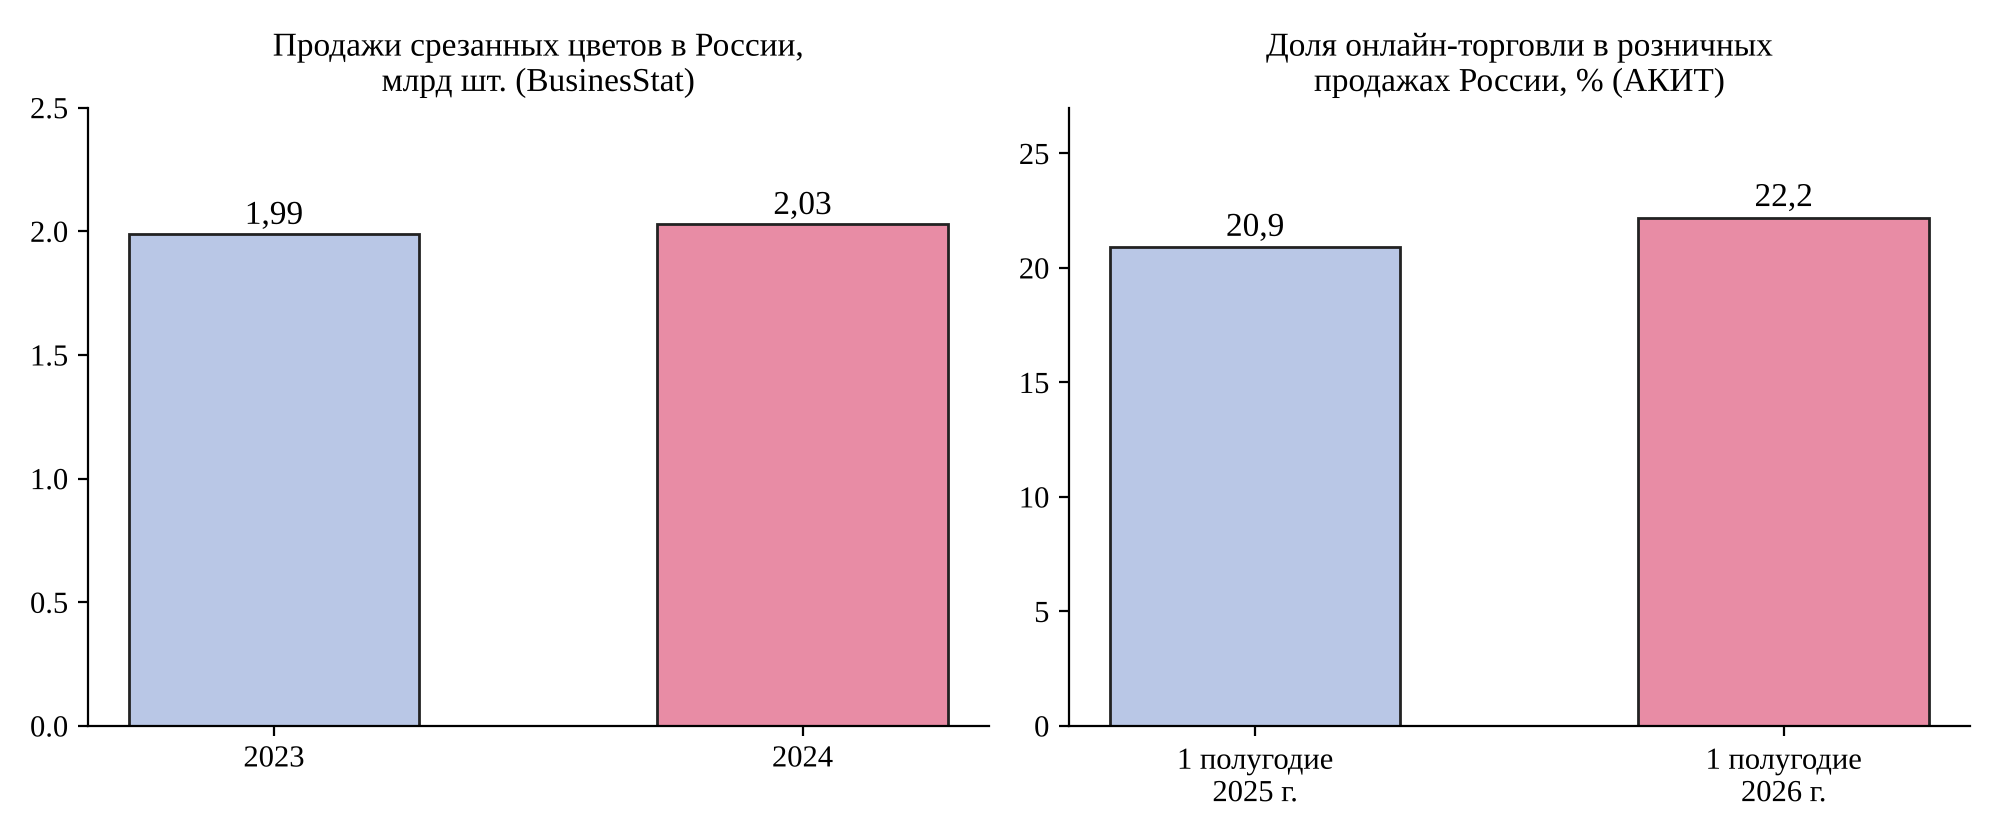
\includegraphics[width=15.5cm,height=0.78\textheight,keepaspectratio]{images/fig01.png}
\caption{Продажи срезанных цветов и~доля онлайн-торговли в~розничных продажах России}\label{fig:1.1}
\end{figure}

Вместе с~тем интернет-торговля остаётся лишь частью рынка: на онлайн-канал приходится 22,2 \% розничных продаж, поэтому основная часть покупок по-прежнему совершается в~традиционных каналах. Это означает, что рынок движется к~омниканальной модели, в~которой магазин использует и~физическую точку, и~цифровые инструменты \cite{b10}.



\subsection{Требования к~приложениям для заказа цветов и~обзор аналогов}

Приложение для заказа цветов относится к~классу систем электронной коммерции, но имеет ряд отличий от универсальных интернет-магазинов. Товар скоропортящийся, поэтому остаток на складе меняется быстро и~должен учитываться в~реальном времени: нельзя допускать оформления заказа на цветы, которых нет в~наличии. Для покупателя важно не только что купить, но и~к~какому времени получить заказ, поэтому выбор даты и~времени самовывоза или доставки является обязательной частью оформления. Спрос носит выраженный сезонный характер с~пиками вокруг праздников, что повышает требования к~устойчивости приложения и~скорости обработки заказов.



С точки зрения пользовательских ролей в~приложении обычно выделяют покупателя и~администратора. Покупатель просматривает каталог, получает подробную информацию о~товаре, формирует корзину и~оформляет заказ. Администратор принимает заказы, меняет их статусы, управляет ценами и~остатками и~анализирует показатели работы магазина. Помимо функциональных, предъявляются нефункциональные требования: удобство использования на экранах разных размеров, приемлемая скорость отклика, сохранность данных, безопасное хранение паролей и~возможность запуска на нескольких платформах из единой кодовой базы.



На российском рынке работает ряд крупных сервисов доставки цветов с~мобильными приложениями. Для анализа выбраны три наиболее показательных представителя разных моделей бизнеса: маркетплейс Flowwow, приложение «Яндекс Цветы», являющееся частью экосистемы крупной технологической компании, и~приложение «Цветов.ру», объединяющее собственные магазины и~партнёров.



Flowwow представляет собой онлайн-маркетплейс, объединяющий продавцов и~покупателей более чем в~1200 городах России и~мира. В~приложении предусмотрены чат с~продавцом для уточнения деталей заказа и~отдельный фильтр магазинов, проверенных сервисом. Приложение развивает 25 товарных категорий, то есть выходит далеко за рамки цветочной тематики. Основной экран приложения показан на рисунке \ref{fig:1.2} \cite{b4}.



\begin{figure}[H]
\centering
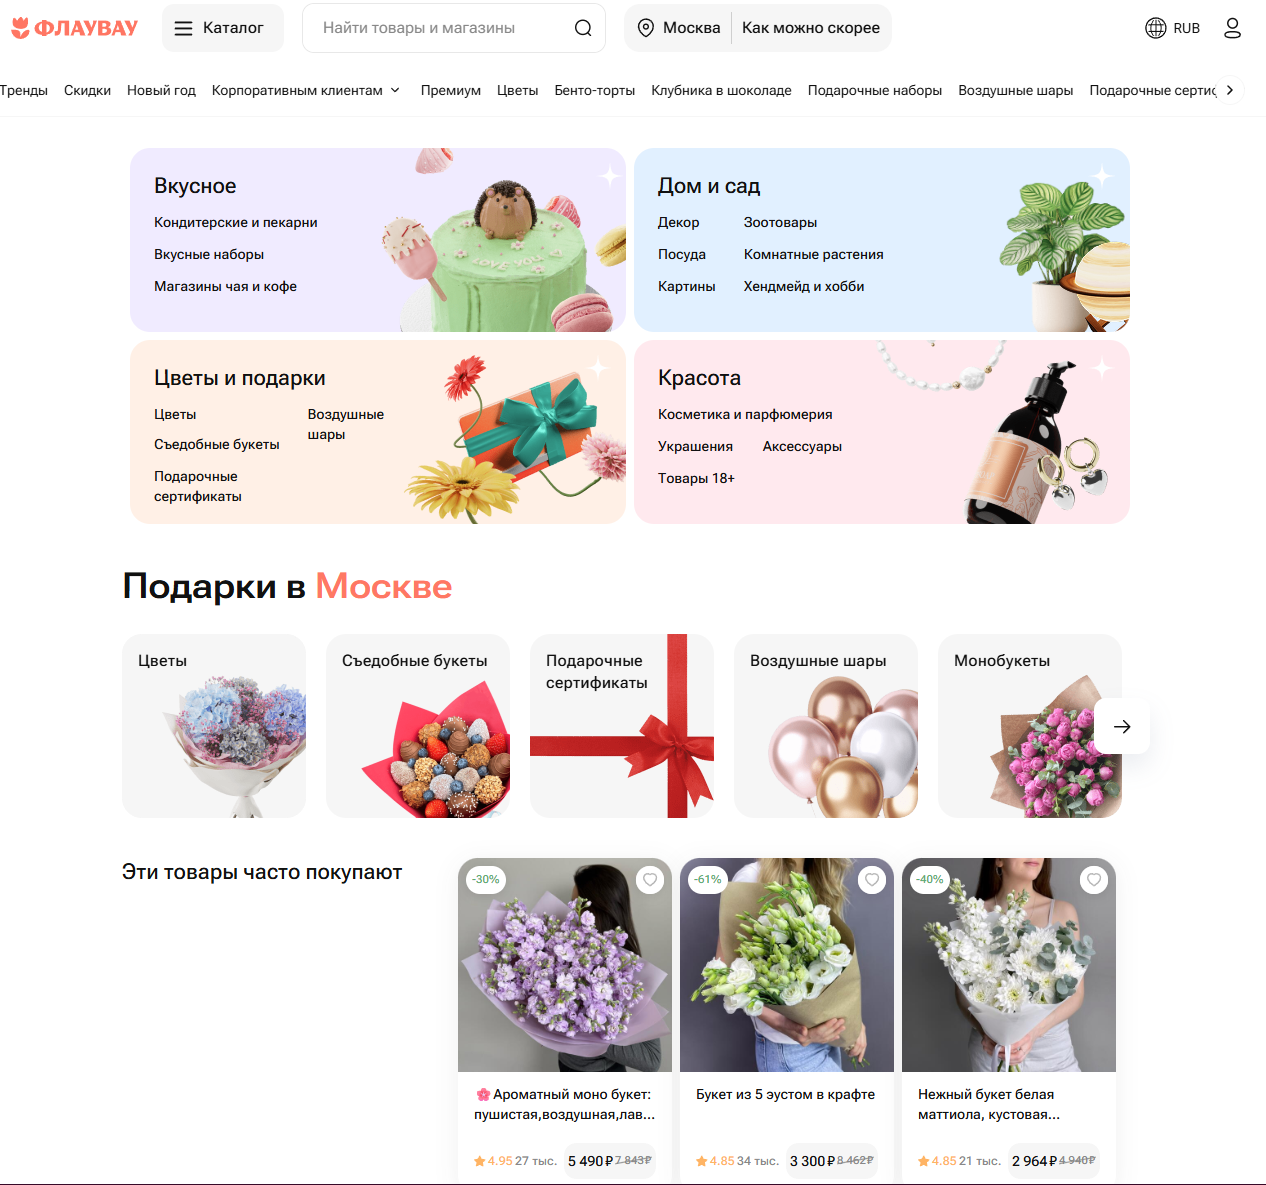
\includegraphics[width=13.8cm,height=0.78\textheight,keepaspectratio]{images/fig02.png}
\caption{Главный экран приложения Flowwow}\label{fig:1.2}
\end{figure}

«Яндекс Цветы»~– приложение сервиса доставки цветов, которое развивает компания «Яндекс». В~каталоге RuStore приложение отображается с~рейтингом 3,4 по 26 оценкам и~более чем 50 тыс. загрузок. Интерфейс приложения показан на рисунке \ref{fig:1.3} \cite{b13}.



\begin{figure}[H]
\centering
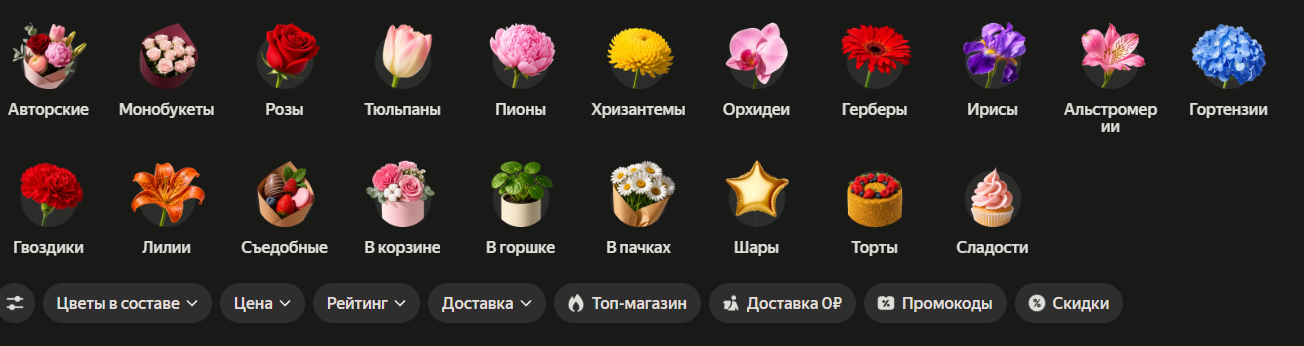
\includegraphics[width=17.0cm,height=0.78\textheight,keepaspectratio]{images/fig03.png}
\caption{Экран приложения «Яндекс Цветы»}\label{fig:1.3}
\end{figure}

«Цветов.ру» работает в~219 городах России, имеет 45 собственных магазинов и~более 370 проверенных партнёров, обеспечивая доставку от 35 минут. Среди особенностей~– обязательная загрузка фотографии собранного заказа магазином до отправки, оплата долями и~разными платёжными методами, кэшбэк и~промокод на первый заказ. В~каталоге RuStore приложение имеет рейтинг 4,7 по 235 оценкам. Экран приложения показан на рисунке \ref{fig:1.4}, а~результаты сравнения сведены в~таблицу \ref{tab:1.1} \cite{b12}.



\begin{figure}[H]
\centering
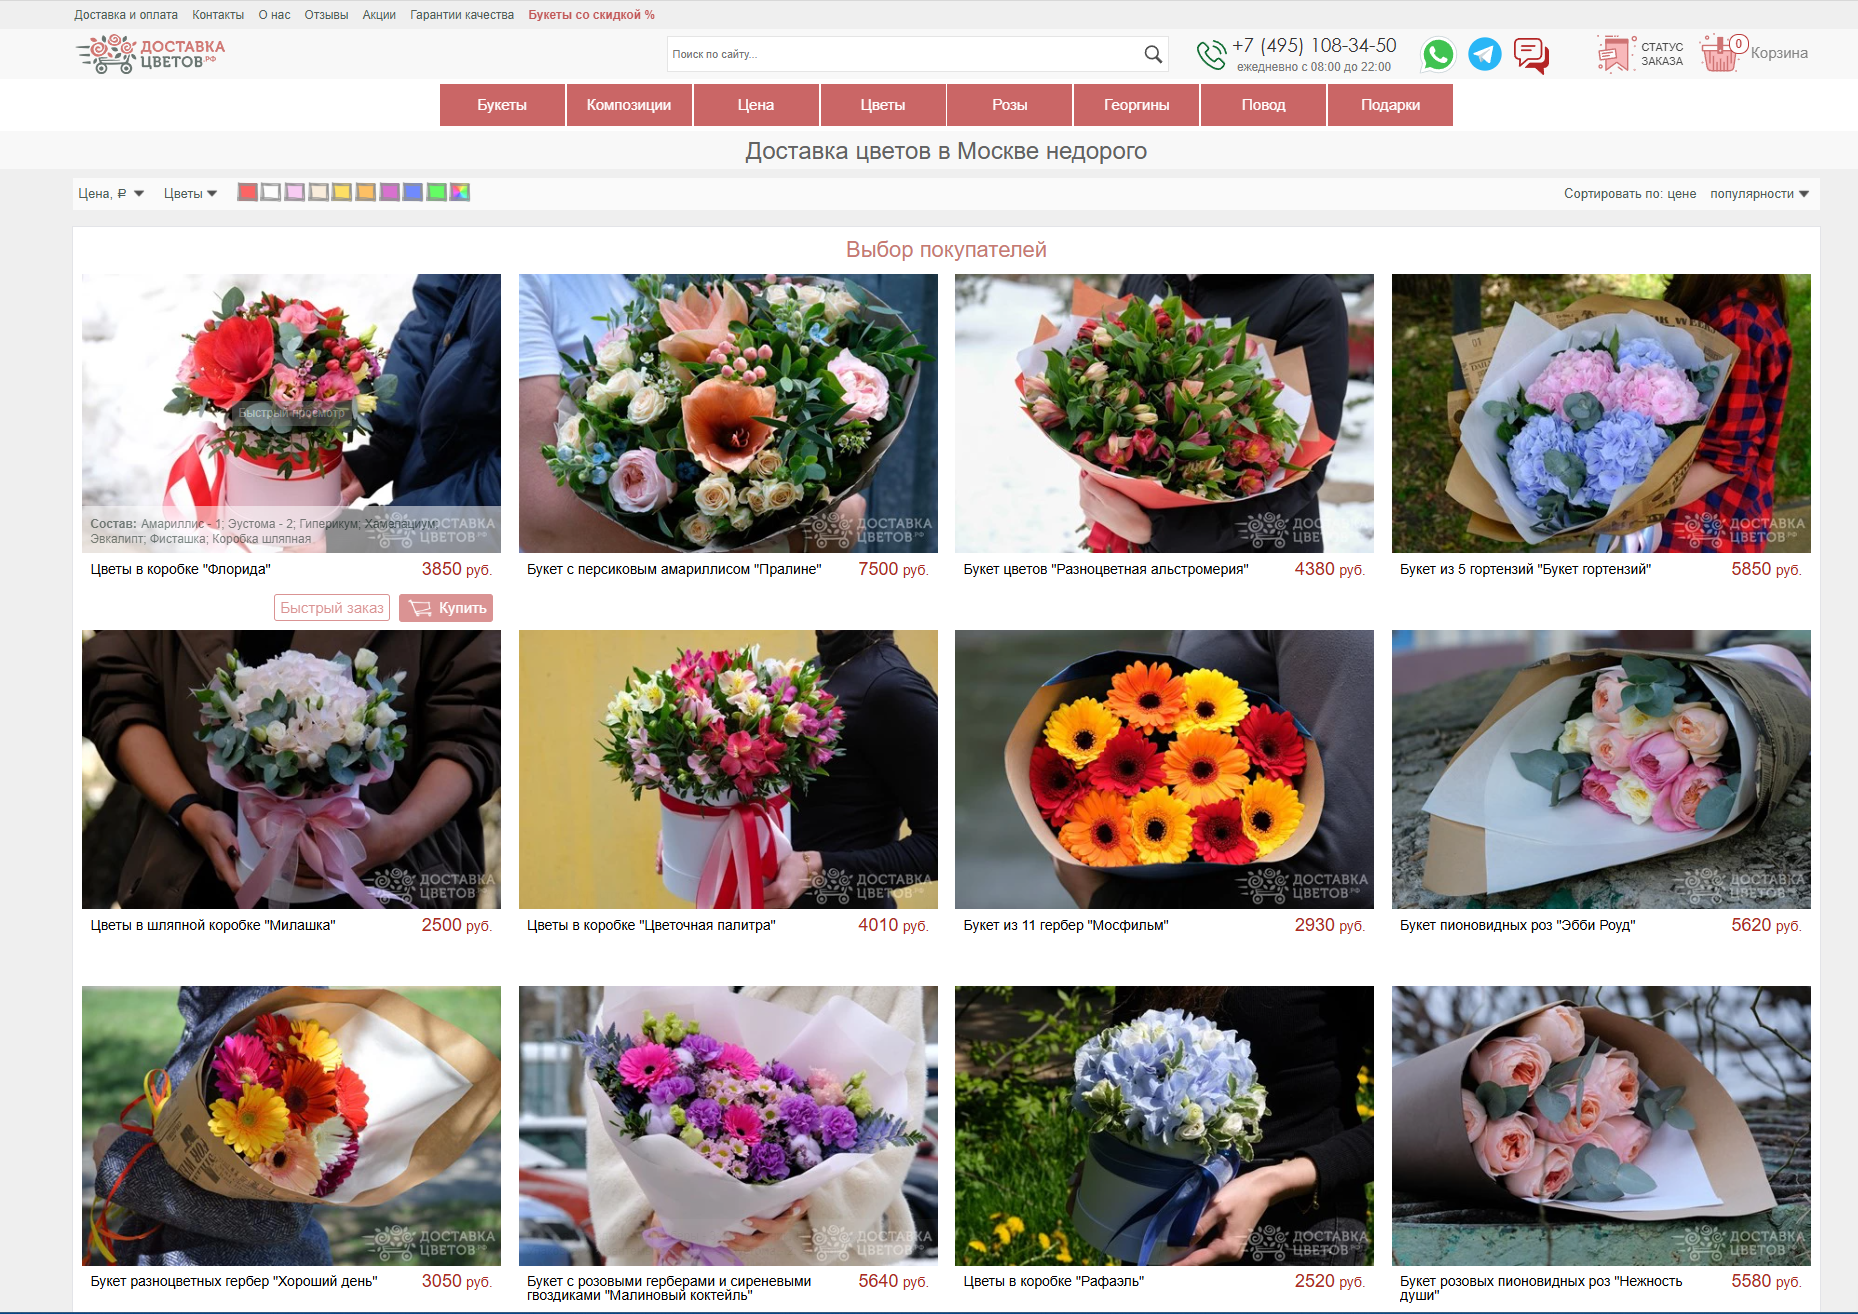
\includegraphics[width=17.0cm,height=0.78\textheight,keepaspectratio]{images/fig04.png}
\caption{Экран приложения «Цветов.ру»}\label{fig:1.4}
\end{figure}

\begingroup\small\singlespacing\setlength{\LTpre}{6pt}\setlength{\LTpost}{10pt}
\begin{longtable}{|>{\raggedright\arraybackslash}p{\dimexpr 0.2241\textwidth-2\tabcolsep-\arrayrulewidth\relax}|>{\raggedright\arraybackslash}p{\dimexpr 0.2587\textwidth-2\tabcolsep-\arrayrulewidth\relax}|>{\raggedright\arraybackslash}p{\dimexpr 0.2587\textwidth-2\tabcolsep-\arrayrulewidth\relax}|>{\raggedright\arraybackslash}p{\dimexpr 0.2586\textwidth-2\tabcolsep-\arrayrulewidth\relax}|}
\caption{Сравнение приложений-аналогов}\label{tab:1.1}\\
\hline
\rowcolor{gray!15}\centering\arraybackslash\bfseries Критерий & \centering\arraybackslash\bfseries Flowwow & \centering\arraybackslash\bfseries Яндекс Цветы & \centering\arraybackslash\bfseries Цветов.ру \\ \hline
\endfirsthead
\hline
\rowcolor{gray!15}\centering\arraybackslash\bfseries Критерий & \centering\arraybackslash\bfseries Flowwow & \centering\arraybackslash\bfseries Яндекс Цветы & \centering\arraybackslash\bfseries Цветов.ру \\ \hline
\endhead
Модель & Маркетплейс продавцов & Сервис в~экосистеме «Яндекса» & Собственные магазины и~партнёры \\ \hline
География & Более 1200 городов России и~мира & По данным источников не уточняется & 219 городов России \\ \hline
Платформы & iOS (App Store) & Android (RuStore) & Android (RuStore) \\ \hline
Особенности & Чат с~продавцом, проверенные магазины, 25 категорий товаров & Развивается компанией «Яндекс» & Фото заказа до доставки, кэшбэк, оплата долями, доставка от 35 минут \\ \hline
Для малого магазина & Работа на условиях площадки & Работа на условиях площадки & Работа на условиях сети \\ \hline
\end{longtable}\endgroup

Анализ показывает, что все рассмотренные приложения ориентированы прежде всего на покупателя, использующего смартфон, и~построены вокруг единой для многих продавцов инфраструктуры. Для небольшого магазина такая модель означает зависимость от правил и~условий площадки. Альтернативой является собственное приложение, в~котором реализован необходимый минимум функций: каталог с~подробной информацией о~цветах и~учётом остатков, корзина, оформление заказа ко времени, а~также рабочее место администратора. Для такого приложения важна возможность запуска как на смартфоне покупателя, так и~на компьютере сотрудника из единой кодовой базы, что приводит к~вопросу выбора подхода к~мультиплатформенной разработке.



\subsection{Подходы к~разработке мультиплатформенных приложений}

Под мультиплатформенным понимают приложение, которое может исполняться в~нескольких операционных системах без полной переработки исходного кода. Выделяют несколько подходов, различающихся способом исполнения кода и~отображения интерфейса.



Нативная разработка предполагает отдельную реализацию для каждой платформы на её основном языке и~с~использованием её стандартных библиотек интерфейса. Такой подход даёт максимальную производительность и~доступ ко всем возможностям платформы, но требует отдельных команд и~кодовых баз. Веб-подход использует браузер как универсальную среду исполнения, однако по условиям задания приложение должно работать на компьютере именно как настольная программа, а~не как веб-страница. Гибридный подход помещает веб-интерфейс в~оболочку, содержащую встроенный браузерный компонент, и~сохраняет зависимость от веб-технологий.



Наиболее подходящим для рассматриваемой задачи является кроссплатформенный подход с~собственным движком отрисовки интерфейса: приложение описывается на одном языке, а~общая библиотека рисует элементы управления самостоятельно, одинаково на всех платформах. К~таким решениям относятся Flutter, Qt и~Kivy. Отдельно стоит подход BeeWare, в~котором один и~тот же код использует нативные виджеты каждой платформы \cite{b2}.



Для задач учебного и~малого коммерческого проекта критичными оказываются порог входа и~простота сборки под обе целевые платформы: чем меньше языков и~инструментов необходимо освоить, тем быстрее можно получить работающее приложение. Поэтому в~центре внимания оказываются решения, позволяющие описать приложение на одном языке программирования и~собирать его под настольные и~мобильные операционные системы единым набором команд. Конкретные средства такого рода для языка Python рассматриваются во второй главе.



\clearpage

\section{ТЕХНОЛОГИИ РАЗРАБОТКИ МУЛЬТИПЛАТФОРМЕННОГО ПРИЛОЖЕНИЯ}

\subsection{Средства создания интерфейса на языке Python}

Python как язык общего назначения удобен для быстрой разработки: он обладает лаконичным синтаксисом, динамической типизацией и~обширной стандартной библиотекой, включающей модуль для работы с~реляционными базами данных SQLite и~средства сетевого взаимодействия. Для построения графического интерфейса на нём разработано несколько библиотек, различающихся способом отрисовки, поддерживаемыми платформами и~способом описания экранов \cite{b7,b11}.



Tkinter входит в~стандартную библиотеку Python и~является интерфейсом к~набору Tcl/Tk. Он прост в~освоении и~подходит для небольших настольных утилит, однако не рассчитан на мобильные платформы, а~внешний вид элементов по умолчанию заметно уступает современным интерфейсам \cite{b7}.



Kivy~– открытый фреймворк для создания приложений с~мультитач-интерфейсом, использующий собственную отрисовку элементов. Пакеты для Android собираются с~помощью инструментов экосистемы Kivy. Интерфейс в~Kivy описывается на Python и~на собственном языке разметки, а~стандартный вид виджетов не следует нативным стилям платформ.



BeeWare~– набор инструментов для создания нативных приложений на Python для настольных и~мобильных платформ. В~нём применяется библиотека виджетов, отображающих элементы нативными средствами каждой ОС. Подход привлекателен привычным видом интерфейса, но экосистема готовых компонентов у~него уже, чем у~фреймворков с~собственным движком \cite{b2}.



Qt for Python (PySide6)~– официальная привязка Python к~библиотеке Qt. Интерфейс можно строить как классическими виджетами, так и~декларативно на языке QML в~рамках технологии Qt Quick, где разметка сцены, привязки свойств и~анимации описываются в~отдельных файлах, а~логика остаётся в~Python. Для взаимодействия между Python и~QML используются сигналы, слоты и~свойства объектов QObject. Сборка под Android выполняется специальным инструментом развёртывания из состава PySide6 и~требует подготовки Android SDK и~NDK \cite{b8}.



Flet~– фреймворк, позволяющий создавать мобильные, настольные и~веб-приложения только на Python: интерфейс описывается объектами Python, а~отрисовка выполняется средствами Flutter. Команда flet build позволяет собирать пакеты для целевых платформ~– Android, iOS, Windows, macOS, Linux и~веб, при этом для сборки необходим Flutter SDK, а~в~документации приведена матрица, показывающая, на какой операционной системе допустимо запускать сборку для каждой целевой платформы. Фреймворк активно развивается, поэтому для воспроизводимости результатов в~разработке фиксируют конкретную версию. Сравнение рассмотренных решений приведено в~таблице \ref{tab:2.1} \cite{b3}.



\begingroup\small\singlespacing\setlength{\LTpre}{6pt}\setlength{\LTpost}{10pt}
\begin{longtable}{|>{\raggedright\arraybackslash}p{\dimexpr 0.1795\textwidth-2\tabcolsep-\arrayrulewidth\relax}|>{\raggedright\arraybackslash}p{\dimexpr 0.2308\textwidth-2\tabcolsep-\arrayrulewidth\relax}|>{\centering\arraybackslash}p{\dimexpr 0.1795\textwidth-2\tabcolsep-\arrayrulewidth\relax}|>{\centering\arraybackslash}p{\dimexpr 0.1795\textwidth-2\tabcolsep-\arrayrulewidth\relax}|>{\raggedright\arraybackslash}p{\dimexpr 0.2308\textwidth-2\tabcolsep-\arrayrulewidth\relax}|}
\caption{Сравнение Python-средств для разработки интерфейса}\label{tab:2.1}\\
\hline
\rowcolor{gray!15}\centering\arraybackslash\bfseries Средство & \centering\arraybackslash\bfseries Основа отрисовки & \centering\arraybackslash\bfseries Настольные ОС & \centering\arraybackslash\bfseries Android & \centering\arraybackslash\bfseries Описание интерфейса \\ \hline
\endfirsthead
\hline
\rowcolor{gray!15}\centering\arraybackslash\bfseries Средство & \centering\arraybackslash\bfseries Основа отрисовки & \centering\arraybackslash\bfseries Настольные ОС & \centering\arraybackslash\bfseries Android & \centering\arraybackslash\bfseries Описание интерфейса \\ \hline
\endhead
Tkinter & Tcl/Tk & \centering\arraybackslash Да & \centering\arraybackslash Нет & Код на Python \\ \hline
Kivy & Собственная отрисовка & \centering\arraybackslash Да & \centering\arraybackslash Да & Python и~язык KV \\ \hline
BeeWare (Toga) & Нативные виджеты ОС & \centering\arraybackslash Да & \centering\arraybackslash Да & Код на Python \\ \hline
PySide6 + QML & Qt Quick & \centering\arraybackslash Да & \centering\arraybackslash Да & QML и~Python \\ \hline
Flet & Flutter & \centering\arraybackslash Да & \centering\arraybackslash Да & Код на Python \\ \hline
\end{longtable}\endgroup

Среди рассмотренных средств наиболее простым для данной задачи является вариант, в~котором интерфейс целиком описывается на Python: он позволяет обойтись одним языком. Технология QML даёт более гибкие возможности оформления, но предполагает знание дополнительного языка и~более сложную настройку сборки под Android. Tkinter не подходит из-за отсутствия мобильной платформы, а~Kivy и~BeeWare требуют более громоздкой подготовки пакетов и~обладают менее богатым набором готовых компонентов для приложений такого типа.



\subsection{Хранение данных и~защита учётных записей}

Данные приложения магазина~– пользователи, товары, заказы, позиции заказов, избранное~– имеют чётко определённую структуру и~связи, поэтому для их хранения подходит реляционная модель. В~ней информация представляется таблицами, строки которых однозначно идентифицируются первичными ключами, а~связи между таблицами задаются внешними ключами. Реляционные системы поддерживают транзакции~– группы операций, которые выполняются как единое целое: либо все, либо ни одной. Это свойство принципиально для оформления заказа, при котором одновременно создаётся запись о~заказе и~уменьшаются остатки товаров.



SQLite~– встраиваемая СУБД, не требующая отдельного серверного процесса и~конфигурирования: база данных хранится в~одном файле и~доступна непосредственно библиотеке, подключённой к~приложению. Разработчики SQLite указывают, что такой подход хорошо подходит для встраиваемых устройств и~приложений, а~также как формат хранения данных приложения. Эти свойства делают SQLite естественным выбором для мультиплатформенного приложения, которое должно работать автономно на разных устройствах. Модуль sqlite3 входит в~стандартную библиотеку Python и~реализует интерфейс DB-API 2.0, включая контекстные менеджеры для управления транзакциями и~параметризованные запросы. Параметризованные запросы, в~которых значения передаются отдельно от текста SQL, защищают приложение от внедрения SQL-кода и~должны применяться везде, где в~запрос подставляются данные пользователя. При использовании базы данных из нескольких потоков (например, интерфейса и~фоновой загрузки изображений) необходимо дополнительно обеспечивать синхронизацию доступа к~единому соединению \cite{b1,b7}.



Аутентификация~– это проверка того, что пользователь является тем, за кого себя выдаёт. Авторизация~– определение того, какие действия ему разрешены. В~приложении магазина достаточно простой ролевой модели (RBAC): каждому пользователю назначается одна роль~– покупатель или администратор,~– а~набор доступных экранов и~операций определяется ролью. Проверку прав необходимо выполнять не только на уровне интерфейса, но и~на уровне логики приложения, чтобы действие нельзя было выполнить в~обход экрана.



Пароли ни при каких условиях не должны храниться в~открытом виде. Организация OWASP в~руководстве по хранению паролей рекомендует использовать специализированные функции формирования ключа с~уникальной случайной солью для каждого пользователя; в~качестве предпочтительного алгоритма называется Argon2id, а~когда требуется совместимость с~FIPS-стандартами, допускается PBKDF2 с~HMAC-SHA-256 при числе итераций не менее 600 000. Соль препятствует использованию заранее вычисленных таблиц хэшей, а~намеренно большая вычислительная стоимость функции замедляет подбор паролей. Сравнение хэшей должно выполняться за постоянное время, чтобы исключить утечки информации через длительность проверки. Кроме того, приложение, которое собирает контактные данные покупателей (имя, телефон, адрес), должно хранить только необходимый минимум сведений и~учитывать требования законодательства о~персональных данных при промышленной эксплуатации \cite{b6}.



\subsection{Получение данных и~изображений из сети}

Современные приложения часто используют данные внешних сервисов, доступных по протоколу HTTP через программный интерфейс (API). Запрос формируется как URL с~параметрами, а~ответ возвращается в~структурированном виде~– чаще всего в~формате JSON, который легко преобразуется в~структуры языка Python средствами стандартной библиотеки. Для приложения магазина это позволяет получать, например, фотографии товаров из открытых источников, не храня их в~составе приложения.



Примером такого сервиса является MediaWiki Action API, предоставляющий программный доступ к~содержимому Википедии. Запрос типа query с~модулем pageimages позволяет получить ссылку на основное изображение статьи заданного размера, причём в~одном запросе можно указать до 50 названий статей, а~сервис возвращает также сведения о~нормализации заголовков и~перенаправлениях, которые необходимо учитывать при сопоставлении результатов. Рекомендации по работе с~публичными API предписывают передавать осмысленный заголовок User-Agent, идентифицирующий приложение, и~не создавать избыточную нагрузку на сервис, поэтому целесообразно объединять названия в~один запрос и~сохранять полученные ссылки, чтобы не повторять запрос при каждом запуске \cite{b5}.



Сетевые операции могут занимать заметное время, поэтому их выполняют в~отдельном потоке, чтобы не блокировать интерфейс: окно приложения открывается сразу, а~изображения подставляются по мере получения данных. При работе с~сетевыми ресурсами необходимо предусматривать отсутствие соединения: приложение не должно прекращать работу, если сервис недоступен, а~пользователь должен видеть осмысленную замену недостающим данным, например цветную заглушку со значком. Изображения, размещённые в~Википедии, распространяются на условиях свободных лицензий, требующих указания источника, поэтому в~интерфейсе следует приводить ссылку на источник фотографий.



Типичная последовательность работы клиента с~таким сервисом включает формирование URL с~кодированием параметров, отправку запроса с~ограничением времени ожидания, разбор ответа в~формате JSON и~проверку наличия нужных полей: сервис может не вернуть изображение для статьи, и~такая ситуация должна обрабатываться как штатная, а~не как ошибка. Исключения сетевого уровня~– недоступность сервера, превышение времени ожидания, ошибки соединения~– перехватываются, а~приложение продолжает работу с~теми данными, которые у~него уже есть. Полученные сведения имеет смысл сохранять в~локальном хранилище, чтобы последующие запуски не зависели от доступности сети. Обмен данными желательно выполнять по защищённому протоколу HTTPS, а~полученные из сети ссылки и~тексты не следует считать доверенными.



\subsection{Выбор технологий для приложения «Флора»}

Выбор технологий определяется требованиями задания: единый язык Python, настольная и~мобильная платформы, отсутствие веб-интерфейса. Из рассмотренных вариантов для основной реализации выбран фреймворк Flet. Интерфейс в~нём описывается Python-объектами, а~отрисовка выполняется средствами Flutter, поэтому всё приложение, включая логику и~интерфейс, написано на одном языке. Сборка под Android и~настольные ОС выполняется единой командой flet build, что соответствует требованию мультиплатформенности. Для воспроизводимости версия фреймворка фиксируется, так как интерфейсы и~способ упаковки могут меняться между выпусками. Для проверки переносимости архитектуры предполагается второй вариант слоя представления~– на PySide6 и~QML \cite{b3,b8}.



Данные хранятся в~SQLite~– встраиваемой базе данных в~одном файле, не требующей сервера. Доступ осуществляется через стандартный модуль sqlite3. Для хранения паролей применяются функции стандартной библиотеки hashlib и~secrets. Загрузка фотографий выполняется стандартным модулем urllib через API Википедии. Модульное тестирование выполняется библиотекой unittest. Перечень технологий приведён в~таблице \ref{tab:2.2} \cite{b1,b5,b7}.



\begingroup\small\singlespacing\setlength{\LTpre}{6pt}\setlength{\LTpost}{10pt}
\begin{longtable}{|>{\raggedright\arraybackslash}p{\dimexpr 0.2778\textwidth-2\tabcolsep-\arrayrulewidth\relax}|>{\raggedright\arraybackslash}p{\dimexpr 0.2963\textwidth-2\tabcolsep-\arrayrulewidth\relax}|>{\raggedright\arraybackslash}p{\dimexpr 0.4259\textwidth-2\tabcolsep-\arrayrulewidth\relax}|}
\caption{Технологический стек приложения}\label{tab:2.2}\\
\hline
\rowcolor{gray!15}\centering\arraybackslash\bfseries Назначение & \centering\arraybackslash\bfseries Технология & \centering\arraybackslash\bfseries Комментарий \\ \hline
\endfirsthead
\hline
\rowcolor{gray!15}\centering\arraybackslash\bfseries Назначение & \centering\arraybackslash\bfseries Технология & \centering\arraybackslash\bfseries Комментарий \\ \hline
\endhead
Язык программирования & Python 3.10 и~выше & Единый язык для интерфейса и~логики \\ \hline
Интерфейс & Flet 0.28.3 (на основе Flutter) & Настольные ОС и~Android из одного кода \\ \hline
Альтернативный интерфейс & PySide6 + QML & Проверка переносимости архитектуры \\ \hline
Хранилище данных & SQLite, модуль sqlite3 & Один файл flora.db, без сервера \\ \hline
Безопасность паролей & hashlib (PBKDF2-HMAC-SHA256), secrets & Случайная соль, сравнение за постоянное время \\ \hline
Сеть & urllib, API Википедии & Поиск и~загрузка фотографий цветов \\ \hline
Тестирование & unittest & Автоматические модульные тесты \\ \hline
Среда разработки & PyCharm & Запуск и~отладка на компьютере \\ \hline
Сборка & flet build apk / windows & Пакеты для Android и~Windows \\ \hline
\end{longtable}\endgroup

\clearpage

\section{РАЗРАБОТКА И~ТЕСТИРОВАНИЕ ПРИЛОЖЕНИЯ «ФЛОРА»}

\subsection{Постановка задачи и~требования к~приложению}

Приложение «Флора» предназначено для небольшого цветочного магазина и~решает две задачи: позволяет покупателю просматривать каталог цветов и~заказывать их с~самовывозом или доставкой к~выбранному времени, а~администратору~– принимать и~обрабатывать заказы, управлять ценами и~остатками. Исходные ограничения определены заданием: приложение разрабатывается на языке Python с~использованием его библиотек, работает на компьютере и~на устройствах Android, содержит не менее 30 видов цветов, поддерживает авторизацию покупателя и~администратора, показывает по каждому цветку подробную информацию, фотографию, среднюю цену и~количество в~наличии; при нулевом остатке отображается, что товара нет в~наличии.



Варианты использования приложения показаны на рисунке \ref{fig:3.1}. Покупатель регистрируется и~входит в~приложение, просматривает каталог с~поиском и~фильтрами, открывает карточку цветка, добавляет цветы в~избранное и~в~корзину, оформляет заказ и~следит за его статусом. Администратор входит под отдельной учётной записью, просматривает текущие заказы, ведёт их выполнение, управляет складом и~просматривает статистику.



\begin{figure}[H]
\centering
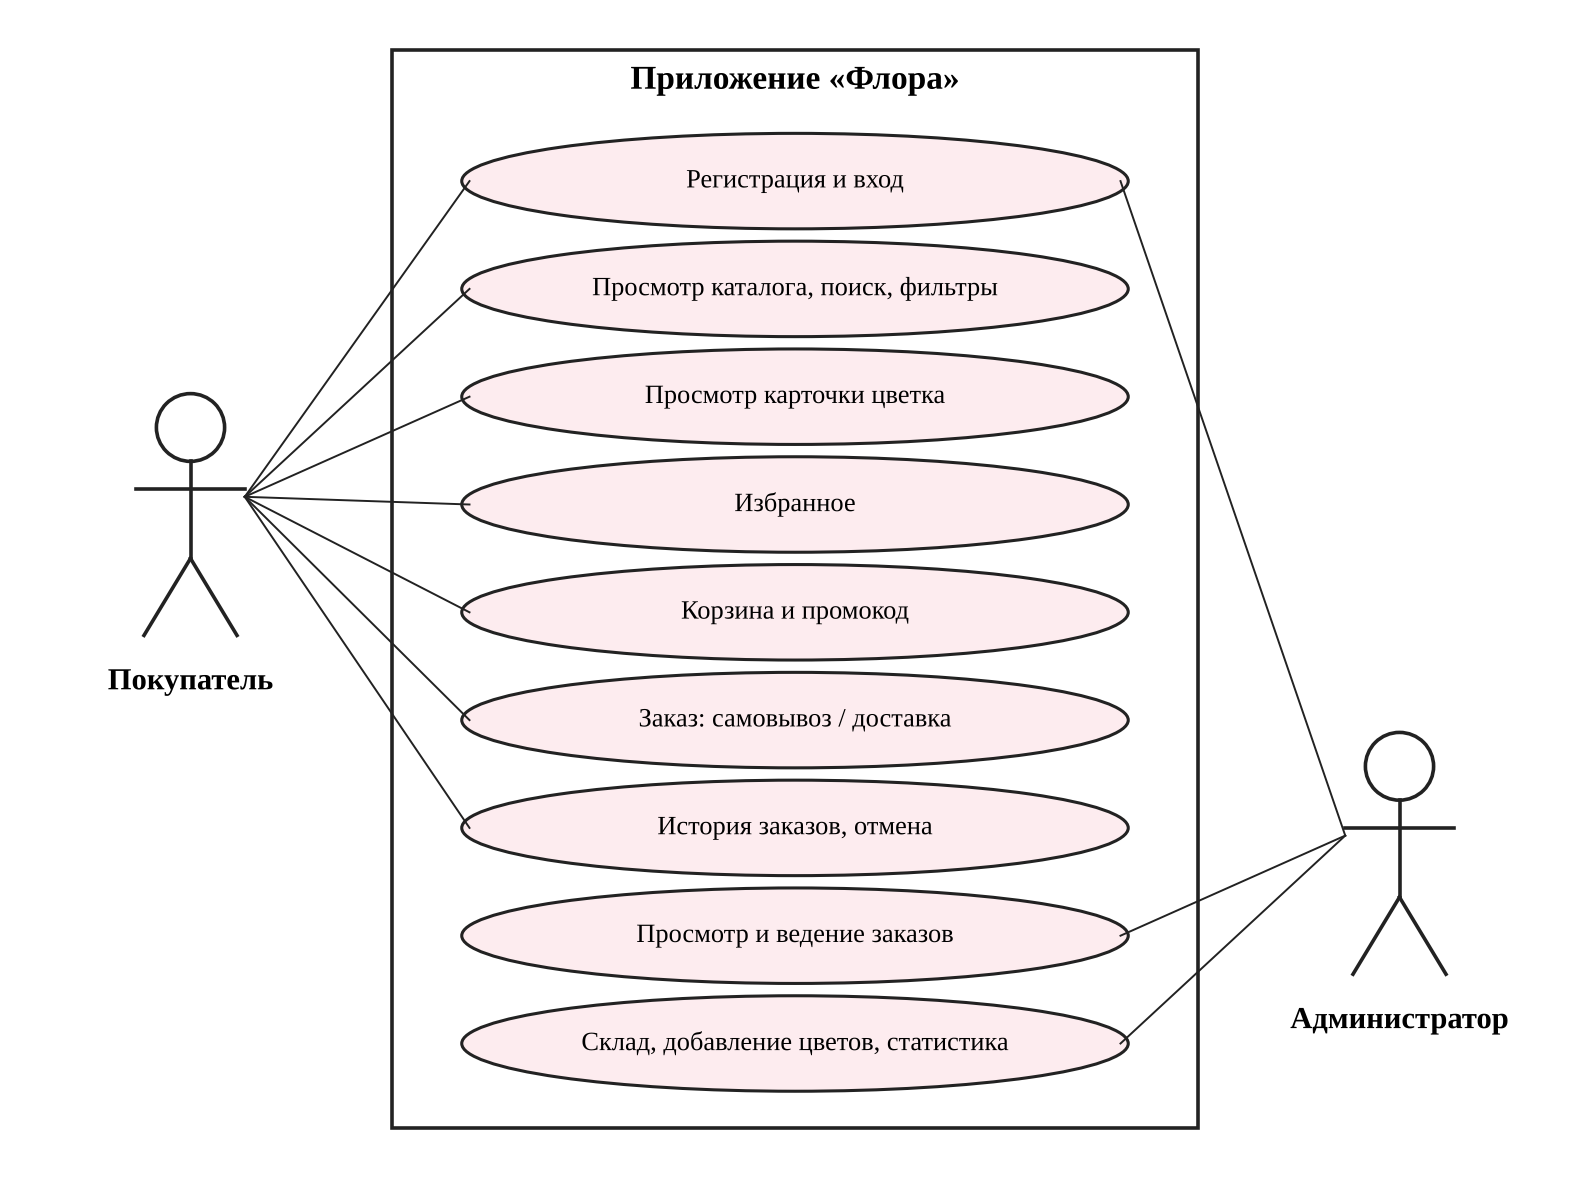
\includegraphics[width=13.5cm,height=0.78\textheight,keepaspectratio]{images/fig05.png}
\caption{Диаграмма вариантов использования приложения «Флора»}\label{fig:3.1}
\end{figure}

Функциональные требования, выделенные по заданию и~по результатам анализа аналогов, сведены в~таблицу \ref{tab:3.1}.



\begingroup\small\singlespacing\setlength{\LTpre}{6pt}\setlength{\LTpost}{10pt}
\begin{longtable}{|>{\centering\arraybackslash}p{\dimexpr 0.1111\textwidth-2\tabcolsep-\arrayrulewidth\relax}|>{\raggedright\arraybackslash}p{\dimexpr 0.6852\textwidth-2\tabcolsep-\arrayrulewidth\relax}|>{\centering\arraybackslash}p{\dimexpr 0.2037\textwidth-2\tabcolsep-\arrayrulewidth\relax}|}
\caption{Функциональные требования}\label{tab:3.1}\\
\hline
\rowcolor{gray!15}\centering\arraybackslash\bfseries Код & \centering\arraybackslash\bfseries Требование & \centering\arraybackslash\bfseries Роль \\ \hline
\endfirsthead
\hline
\rowcolor{gray!15}\centering\arraybackslash\bfseries Код & \centering\arraybackslash\bfseries Требование & \centering\arraybackslash\bfseries Роль \\ \hline
\endhead
\centering\arraybackslash FR-01 & Регистрация покупателя и~вход по логину и~паролю; отдельная учётная запись администратора & \centering\arraybackslash Все \\ \hline
\centering\arraybackslash FR-02 & Каталог не менее чем из 30 видов цветов, разбитых на категории & \centering\arraybackslash Покупатель \\ \hline
\centering\arraybackslash FR-03 & Поиск по названию, фильтр по категории, сортировка по названию, цене и~наличию & \centering\arraybackslash Покупатель \\ \hline
\centering\arraybackslash FR-04 & Карточка цветка фото, латинское название, почва, подкормка, период цветения, высота, освещение, полив, срок в~вазе, символика, интересный факт, цена, остаток & \centering\arraybackslash Покупатель \\ \hline
\centering\arraybackslash FR-05 & Фотографии цветков загружаются из интернета & \centering\arraybackslash Все \\ \hline
\centering\arraybackslash FR-06 & Отображение остатка; при нулевом остатке~– «Нет в~наличии» и~запрет добавления в~корзину & \centering\arraybackslash Покупатель \\ \hline
\centering\arraybackslash FR-07 & Избранное добавление и~удаление цветка, отдельный экран & \centering\arraybackslash Покупатель \\ \hline
\centering\arraybackslash FR-08 & Корзина изменение количества, удаление позиций, расчёт итоговой суммы & \centering\arraybackslash Покупатель \\ \hline
\centering\arraybackslash FR-09 & Оформление заказа самовывоз либо доставка; выбор даты и~времени; телефон, адрес, комментарий & \centering\arraybackslash Покупатель \\ \hline
\centering\arraybackslash FR-10 & Промокоды и~бесплатная доставка при достижении порога суммы & \centering\arraybackslash Покупатель \\ \hline
\centering\arraybackslash FR-11 & История заказов со статусами, отмена нового заказа & \centering\arraybackslash Покупатель \\ \hline
\centering\arraybackslash FR-12 & Просмотр текущих заказов и~их выполнения, фильтр по статусам & \centering\arraybackslash Администратор \\ \hline
\centering\arraybackslash FR-13 & Смена статуса заказа (Новый \ensuremath{\rightarrow} В~работе \ensuremath{\rightarrow} Готов \ensuremath{\rightarrow} Завершён) и~отмена с~возвратом товара на склад & \centering\arraybackslash Администратор \\ \hline
\centering\arraybackslash FR-14 & Управление складом изменение цены, остатка и~ссылки на фото; добавление новых цветов & \centering\arraybackslash Администратор \\ \hline
\centering\arraybackslash FR-15 & Статистика выручка, число заказов, средний чек, популярные цветы, товары на исходе & \centering\arraybackslash Администратор \\ \hline
\end{longtable}\endgroup

К нефункциональным требованиям отнесены: работа из единой кодовой базы на компьютере и~на Android, адаптивность интерфейса к~размеру окна и~экрана, хранение паролей только в~виде хэшей, сохранность данных между запусками, устойчивость к~отсутствию интернета (фото заменяются значками), понятные русскоязычные сообщения об ошибках и~отклик на типовые операции не более долей секунды.



\subsection{Архитектура приложения и~проектирование базы данных}

Приложение построено по слоистой схеме с~разделением ответственности между модулями, что упрощает сопровождение и~тестирование. Верхний слой~– слой представления: он реализован в~модуле main.py классом App, который строит экраны и~обрабатывает действия пользователя. Средний слой~– логика и~доступ к~данным в~модуле db.py: функции аутентификации, оформления заказов, учёта склада и~расчёта стоимости не зависят от библиотеки интерфейса и~поэтому могут проверяться автоматическими тестами без запуска окна. Нижний слой~– база данных SQLite. Отдельно выделен модуль photos.py, который обращается к~интернет-сервису для получения ссылок на фотографии. Структура приложения показана на рисунке \ref{fig:3.2}.



\begin{figure}[H]
\centering
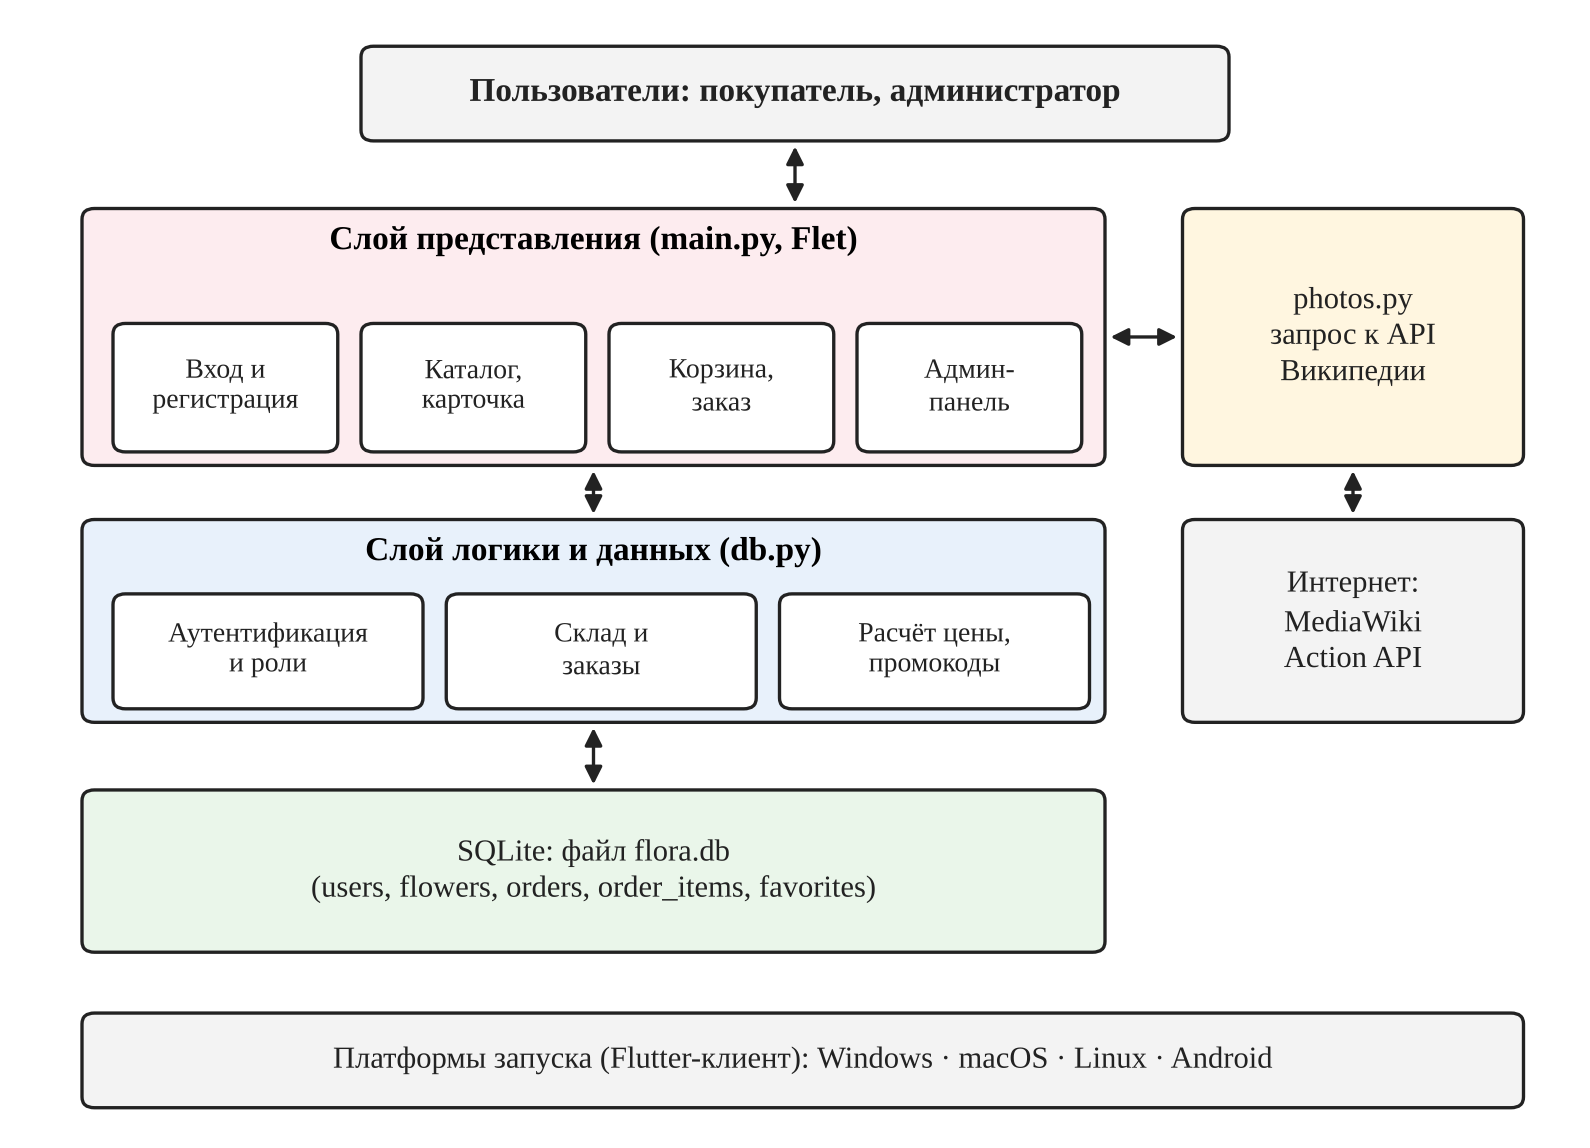
\includegraphics[width=13.5cm,height=0.78\textheight,keepaspectratio]{images/fig06.png}
\caption{Архитектура приложения «Флора»}\label{fig:3.2}
\end{figure}

Данные приложения хранятся в~пяти таблицах. Таблица users содержит учётные записи и~роль пользователя (customer или admin), таблица flowers~– каталог с~описанием ухода, ценой, остатком и~ссылкой на фотографию, таблицы orders и~order\_\allowbreak{}items~– заказы и~их позиции, таблица favorites~– избранное. Связи между таблицами показаны на рисунке \ref{fig:3.3}.



\begin{figure}[H]
\centering
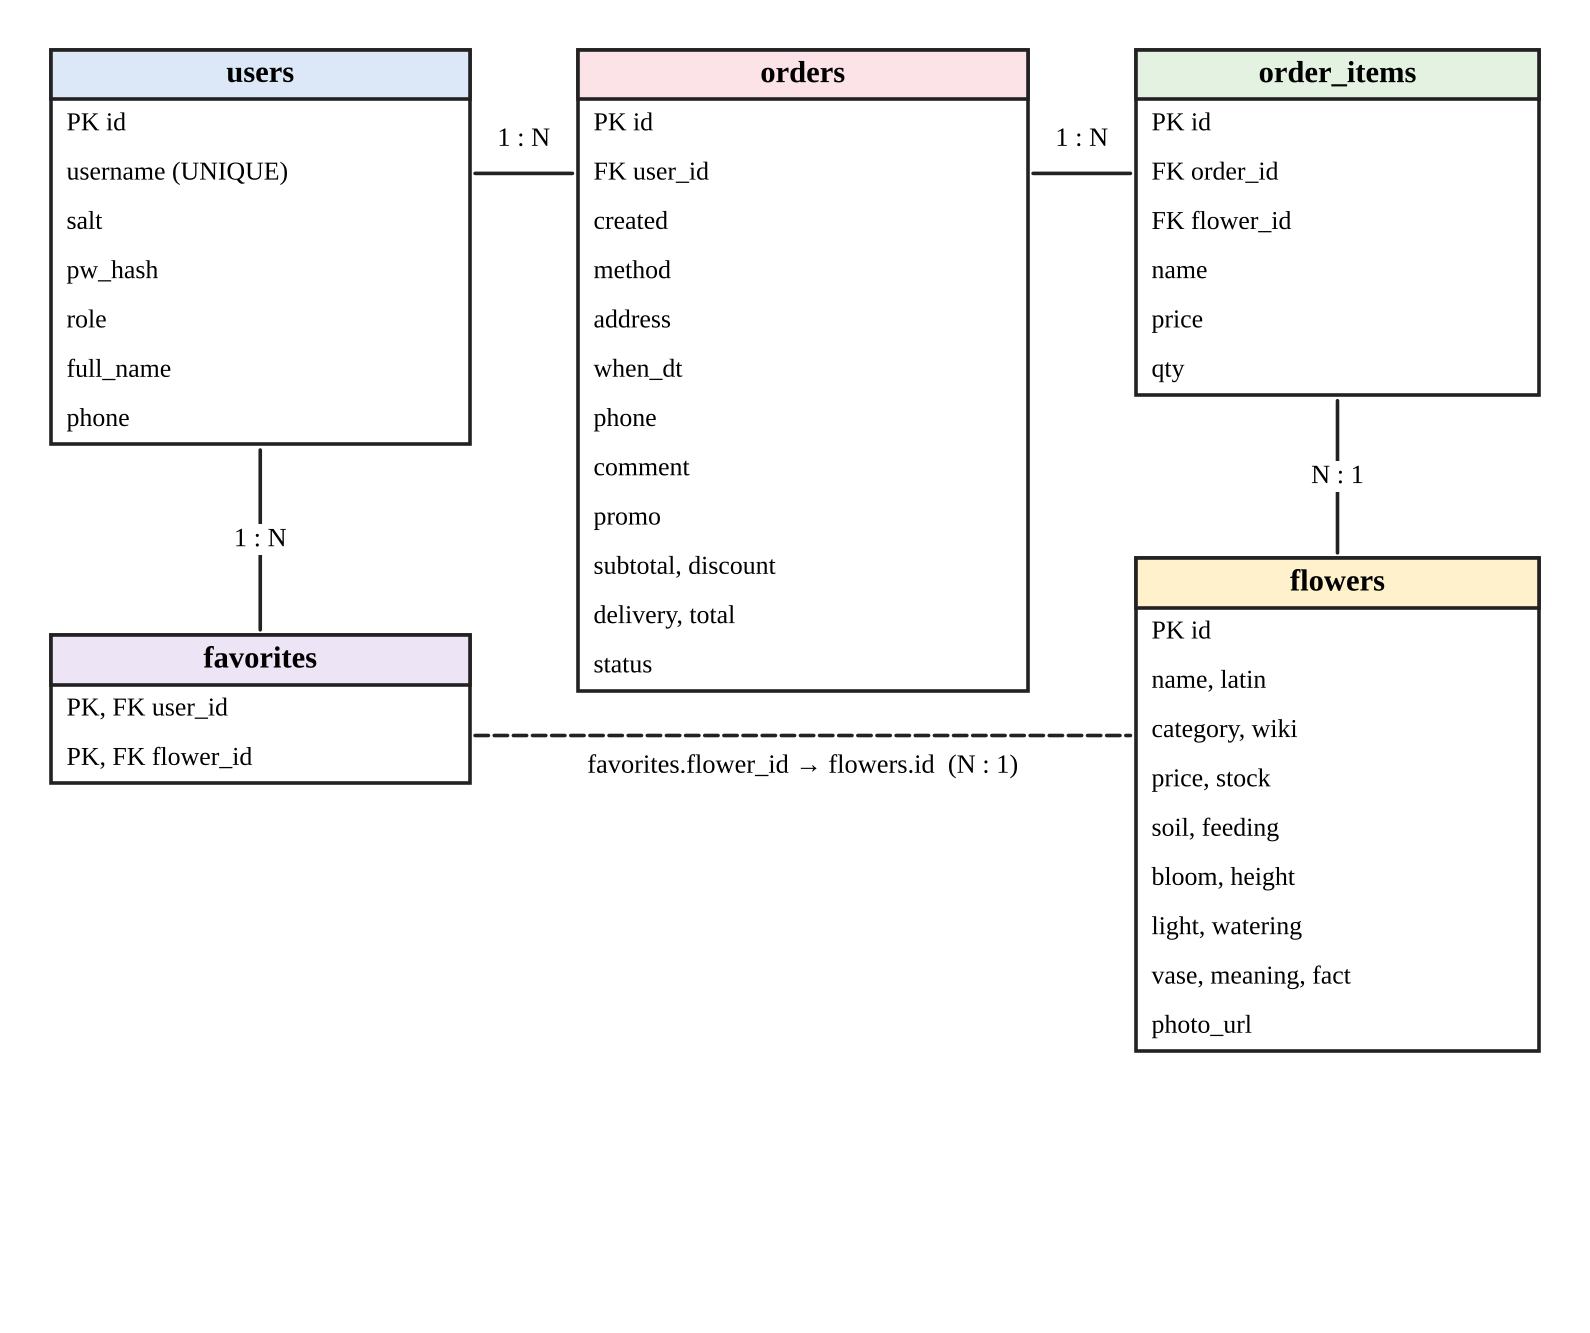
\includegraphics[width=14.0cm,height=0.78\textheight,keepaspectratio]{images/fig07.png}
\caption{Схема базы данных (ER-диаграмма)}\label{fig:3.3}
\end{figure}

Название и~цена цветка копируются в~таблицу order\_\allowbreak{}items в~момент оформления заказа. Это позволяет сохранять историю заказов неизменной, даже если администратор позднее изменит цену или удалит позицию из каталога.



При первом запуске приложение создаёт таблицы, заполняет каталог данными из модуля flowers\_\allowbreak{}data.py и~создаёт учётную запись администратора. Цены в~каталоге заданы средними розничными значениями в~диапазоне от 25 до 1800 рублей за стебель, горшок или ветку, а~остатки~– демонстрационными. Четыре позиции намеренно имеют нулевой остаток, чтобы показать поведение приложения при отсутствии товара.



\subsection{Реализация логики приложения}

Пароль пользователя никогда не сохраняется в~открытом виде. При регистрации генерируется случайная соль длиной 16 байт, после чего функция pbkdf2\_\allowbreak{}hmac библиотеки hashlib вычисляет хэш пароля алгоритмом PBKDF2 с~HMAC-SHA-256 и~120 000 итераций; в~таблицу записываются соль и~хэш. При входе хэш пересчитывается с~сохранённой солью и~сравнивается с~записанным функцией compare\_\allowbreak{}digest, выполняющей сравнение за постоянное время. Такая схема соответствует рекомендациям по хранению паролей: применяется специализированная функция формирования ключа с~уникальной солью. Реализация показана на рисунках \ref{fig:3.4} и~\ref{fig:3.5} \cite{b6}.



\begin{figure}[H]
\centering
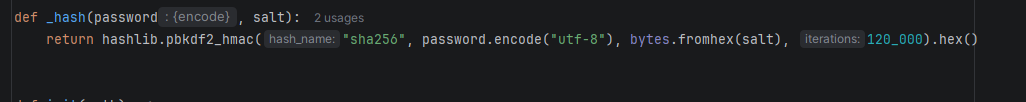
\includegraphics[width=17.0cm,height=0.78\textheight,keepaspectratio]{images/fig08.png}
\caption{Хэширование пароля и~проверка входа}\label{fig:3.4}
\end{figure}

\begin{figure}[H]
\centering
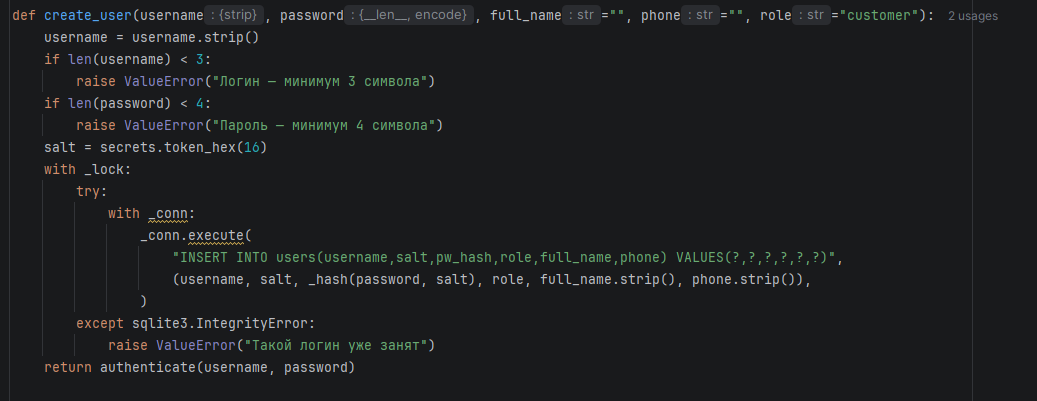
\includegraphics[width=17.0cm,height=0.78\textheight,keepaspectratio]{images/fig09.png}
\caption{Регистрация пользователя}\label{fig:3.5}
\end{figure}

Роль пользователя определяется полем role. После успешного входа приложение показывает разные наборы экранов: покупателю~– «Каталог», «Избранное», «Корзина», «Заказы» и~«Профиль», администратору~– «Заказы», «Цветы», «Статистика» и~«Профиль». Права проверяются и~на уровне логики: смена статуса заказа и~правка цен доступны только администратору. Права доступа к~функциям сведены в~таблице \ref{tab:3.2}.



\begingroup\small\singlespacing\setlength{\LTpre}{6pt}\setlength{\LTpost}{10pt}
\begin{longtable}{|>{\raggedright\arraybackslash}p{\dimexpr 0.5555\textwidth-2\tabcolsep-\arrayrulewidth\relax}|>{\centering\arraybackslash}p{\dimexpr 0.2222\textwidth-2\tabcolsep-\arrayrulewidth\relax}|>{\centering\arraybackslash}p{\dimexpr 0.2222\textwidth-2\tabcolsep-\arrayrulewidth\relax}|}
\caption{Распределение прав доступа по ролям}\label{tab:3.2}\\
\hline
\rowcolor{gray!15}\centering\arraybackslash\bfseries Действие & \centering\arraybackslash\bfseries Покупатель & \centering\arraybackslash\bfseries Администратор \\ \hline
\endfirsthead
\hline
\rowcolor{gray!15}\centering\arraybackslash\bfseries Действие & \centering\arraybackslash\bfseries Покупатель & \centering\arraybackslash\bfseries Администратор \\ \hline
\endhead
Просмотр каталога и~карточек & \centering\arraybackslash Да & \centering\arraybackslash Да (через склад) \\ \hline
Избранное, корзина, оформление заказа & \centering\arraybackslash Да & \centering\arraybackslash Нет \\ \hline
Просмотр собственных заказов и~отмена нового заказа & \centering\arraybackslash Да & \centering\arraybackslash Нет \\ \hline
Просмотр заказов всех покупателей & \centering\arraybackslash Нет & \centering\arraybackslash Да \\ \hline
Смена статуса заказа, отмена любого активного заказа & \centering\arraybackslash Нет & \centering\arraybackslash Да \\ \hline
Изменение цен, остатков, добавление цветов & \centering\arraybackslash Нет & \centering\arraybackslash Да \\ \hline
Просмотр статистики & \centering\arraybackslash Нет & \centering\arraybackslash Да \\ \hline
\end{longtable}\endgroup

Оформление заказа~– наиболее ответственная операция: в~ней одновременно проверяется наличие товара, считается стоимость, создаётся запись о~заказе и~уменьшается остаток. Функция place\_\allowbreak{}order выполняет её как единую транзакцию: сначала проверяется, что каждой позиции корзины хватает на складе, затем в~блоке with подключения к~базе данных создаются запись заказа и~его позиции и~уменьшаются остатки. Если любая проверка не пройдена, генерируется исключение с~понятным сообщением, а~изменения не записываются (рисунок \ref{fig:3.6}).



\begin{figure}[H]
\centering
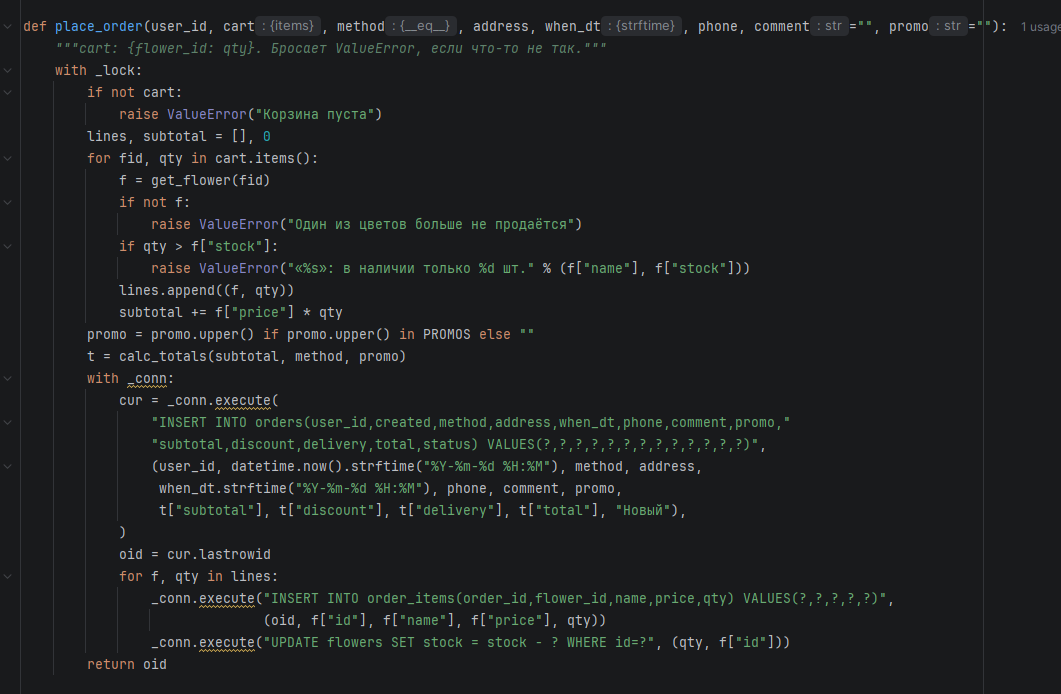
\includegraphics[width=14.5cm,height=0.78\textheight,keepaspectratio]{images/fig10.png}
\caption{Оформление заказа как единая транзакция}\label{fig:3.6}
\end{figure}

Стоимость вычисляется функцией calc\_\allowbreak{}totals (рисунок \ref{fig:3.7}). Скидка по промокоду считается от суммы цветов; поддерживаются коды SPRING10 (10 \%), FLORA15 (15 \%) и~HELLO5 (5 \%). Доставка стоит 300 рублей и~становится бесплатной, если сумма заказа после скидки не меньше 3000 рублей; при самовывозе она не взимается.



\begin{figure}[H]
\centering
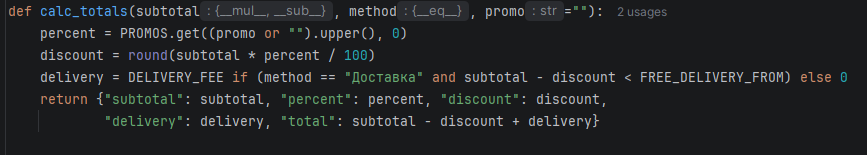
\includegraphics[width=17.0cm,height=0.78\textheight,keepaspectratio]{images/fig11.png}
\caption{Расчёт стоимости заказа}\label{fig:3.7}
\end{figure}

Заказ проходит через статусы «Новый», «В работе», «Готов» и~«Завершён». Из любого незавершённого состояния его можно отменить, как показано на рисунке \ref{fig:3.8}. Закрытые заказы изменять нельзя. При отмене товар возвращается на склад, что реализовано в~функции set\_\allowbreak{}order\_\allowbreak{}status (рисунок \ref{fig:3.9}).



\begin{figure}[H]
\centering
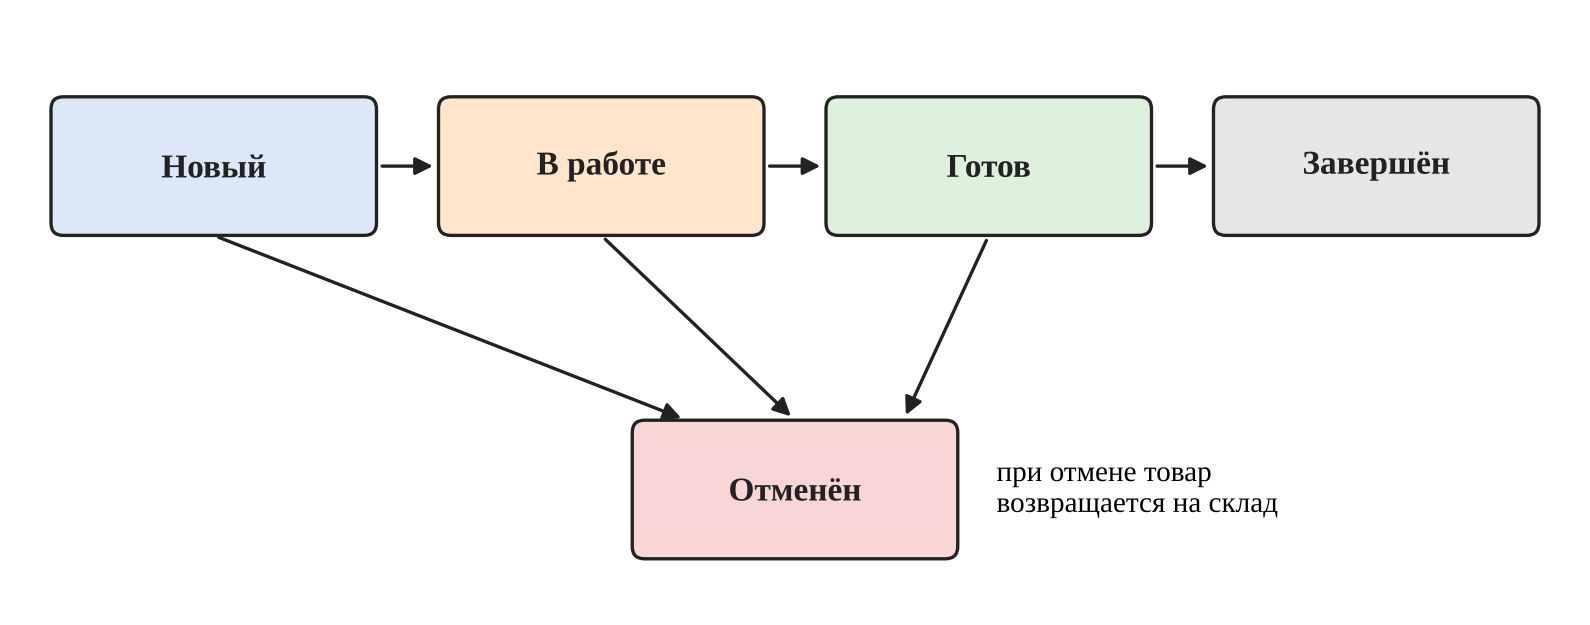
\includegraphics[width=15.0cm,height=0.78\textheight,keepaspectratio]{images/fig12.png}
\caption{Диаграмма статусов заказа}\label{fig:3.8}
\end{figure}

\begin{figure}[H]
\centering
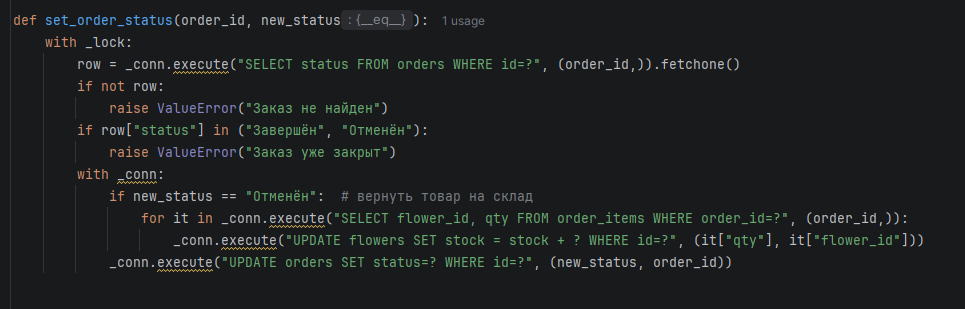
\includegraphics[width=16.9cm,height=0.78\textheight,keepaspectratio]{images/fig13.png}
\caption{Смена статуса заказа с~возвратом товара на склад}\label{fig:3.9}
\end{figure}

Согласно заданию, фотографии цветов берутся из интернета. Для этого используется API Википедии: в~модуле flowers\_\allowbreak{}data.py каждому цветку сопоставлено название статьи в~английской Википедии, а~модуль photos.py одним запросом получает ссылки на основные изображения этих статей. Запрос выполняется с~параметрами prop=pageimages и~pithumbsize=500, то есть запрашиваются миниатюры шириной до 500 пикселей. Названия объединяются в~группы по 40 штук, что укладывается в~ограничение сервиса. Ответ содержит сведения о~нормализации названий и~перенаправлениях, поэтому для сопоставления результатов с~исходными названиями функция последовательно применяет эти соответствия (рисунок \ref{fig:3.10}) \cite{b5}.



\begin{figure}[H]
\centering
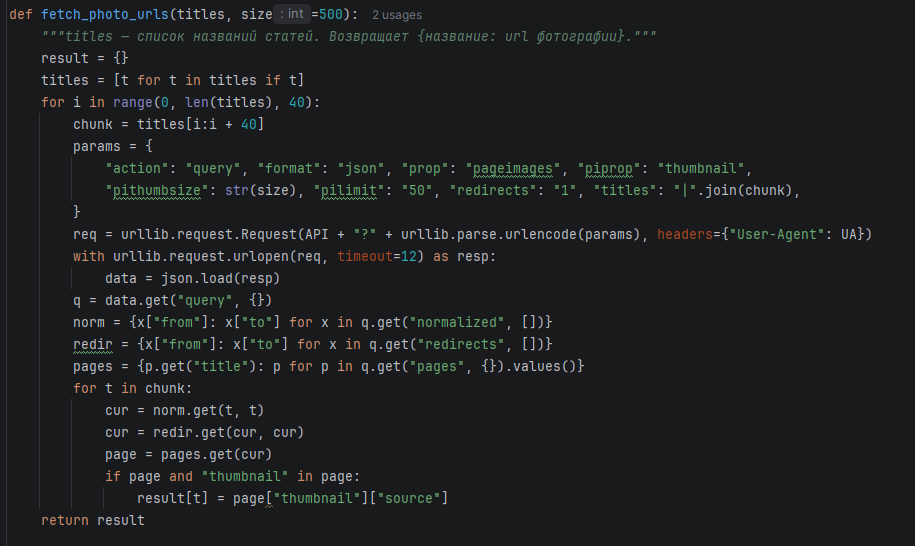
\includegraphics[width=17.0cm,height=0.78\textheight,keepaspectratio]{images/fig14.png}
\caption{Получение ссылок на фотографии через API Википедии}\label{fig:3.10}
\end{figure}

Загрузка запускается в~отдельном потоке при старте приложения, чтобы не задерживать показ интерфейса, и~выполняется только для цветов, у~которых ссылка на фото ещё не сохранена. Найденные ссылки записываются в~поле photo\_\allowbreak{}url таблицы flowers, поэтому при следующих запусках запрос не повторяется. Фотографии отображаются элементом Image, которому в~качестве источника передаётся адрес изображения. Пока фото не загружено или интернет недоступен, вместо него показывается цветная заглушка со значком категории; когда ссылка находится, уже построенные элементы обновляются на месте. Администратор может вручную заменить ссылку на фото в~карточке склада или повторить поиск недостающих фотографий.



\subsection{Реализация пользовательского интерфейса}

После входа покупатель попадает в~основной экран с~нижней панелью навигации из пяти вкладок. Такой шаблон хорошо знаком пользователям мобильных приложений и~одинаково работает в~окне компьютера. Экран входа и~регистрации (рисунок \ref{fig:3.11}) содержит поля логина и~пароля; при регистрации дополнительно запрашиваются имя и~телефон; сообщения об ошибках отображаются под полями.



\begin{figure}[H]
\centering
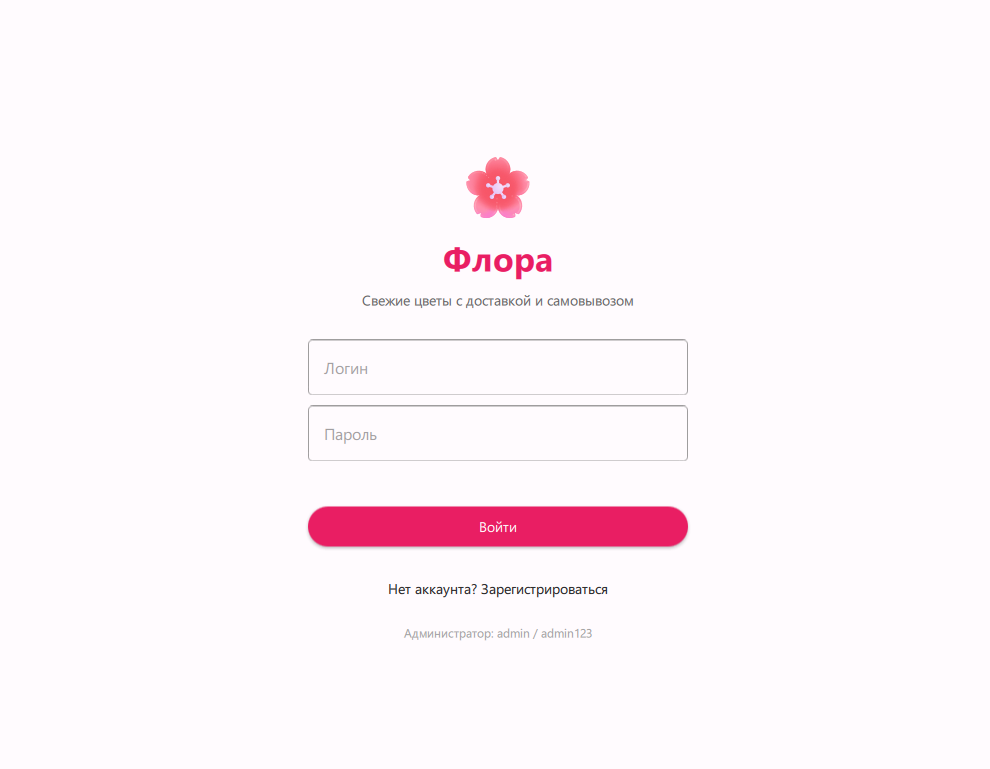
\includegraphics[width=14.3cm,height=0.78\textheight,keepaspectratio]{images/fig15.png}
\caption{Экран входа и~регистрации}\label{fig:3.11}
\end{figure}

Каталог (рисунок \ref{fig:3.12}) показывает цветы плитками в~адаптивной сетке. Количество колонок определяется шириной окна: каждая плитка имеет максимальную ширину около 210 пикселей, поэтому на широком окне компьютера отображается несколько колонок, а~на экране телефона~– одна или две. Над сеткой расположены строка поиска, выбор категории и~сортировки. Плитка содержит фотографию, название, категорию, цену, остаток и~кнопку избранного; для цветов без остатка надпись «Нет в~наличии» выделена красным, а~плитка затемнена.



\begin{figure}[H]
\centering
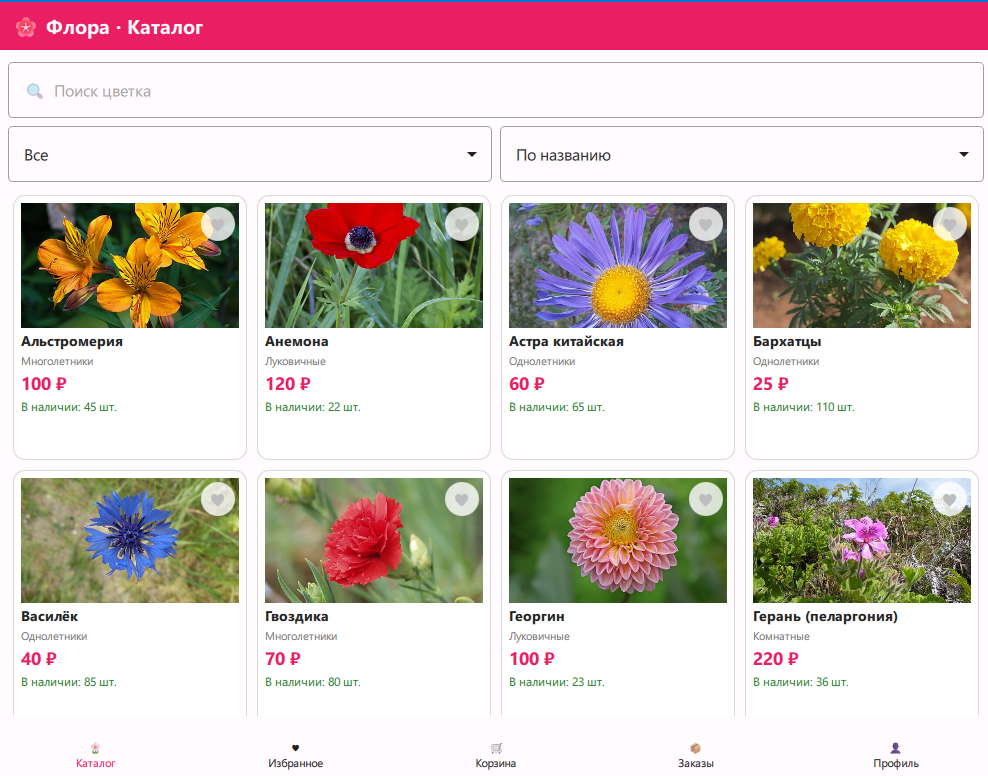
\includegraphics[width=14.4cm,height=0.78\textheight,keepaspectratio]{images/fig16.png}
\caption{Каталог цветов}\label{fig:3.12}
\end{figure}

При нажатии на плитку открывается окно с~подробной информацией о~цветке (рисунок \ref{fig:3.13}). В~нём приведены фотография, латинское название, категория, цена, наличие, а~также девять информационных блоков: почва, чем подкармливать, период цветения, высота растения, освещение, полив, срок в~вазе, что символизирует цветок и~интересный факт. Это превышает минимальный набор сведений, указанный в~задании. Внизу окна находится выбор количества и~кнопка «В корзину»; если остаток равен нулю или весь остаток уже находится в~корзине, кнопка блокируется, а~статус сообщает об этом.



\begin{figure}[H]
\centering
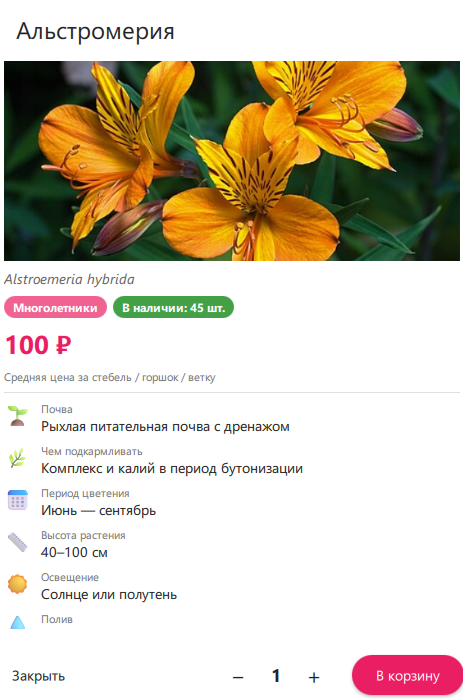
\includegraphics[width=8.3cm,height=0.78\textheight,keepaspectratio]{images/fig17.png}
\caption{Окно с~подробной информацией о~цветке}\label{fig:3.13}
\end{figure}

Вкладка «Избранное» повторяет каталог, но показывает только отмеченные цветы. Вкладка «Корзина» (рисунок \ref{fig:3.14}) содержит список позиций с~изменением количества и~удалением, а~ниже~– форму оформления заказа: переключатель «Самовывоз / Доставка», поле адреса, выбор даты на ближайшие 14 дней и~времени с~шагом 30 минут в~часы работы магазина с~9:00 до 20:00, телефон, комментарий и~промокод, а~также блок итоговой суммы со скидкой и~стоимостью доставки. Список доступного времени строится с~учётом текущего момента: для сегодняшней даты предлагаются только слоты, до которых остаётся не менее часа.



\begin{figure}[H]
\centering
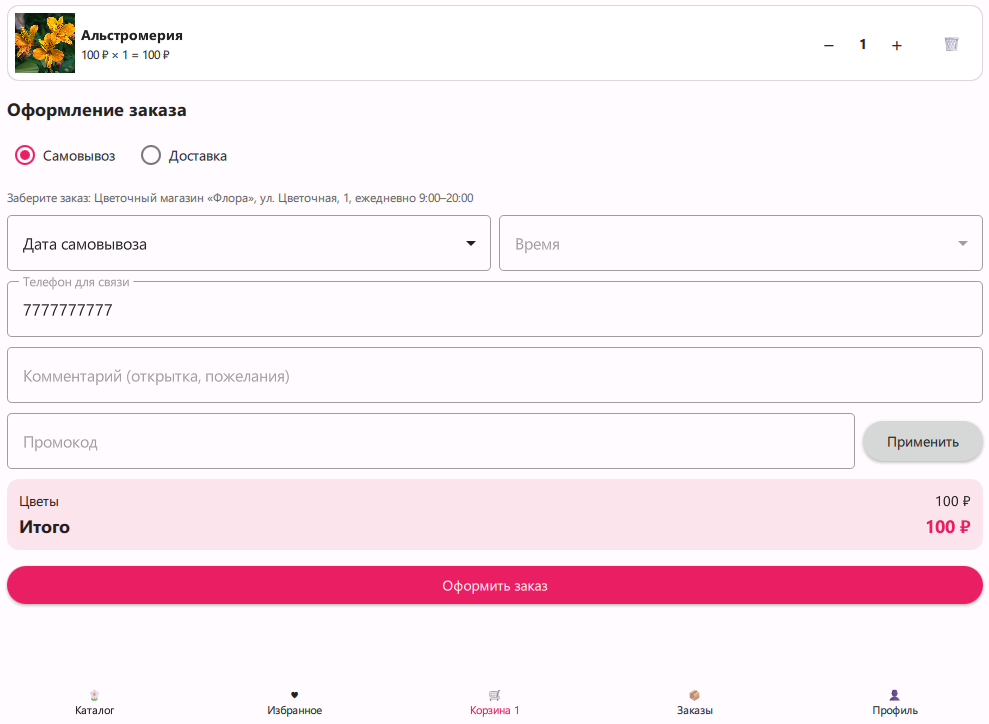
\includegraphics[width=13.7cm,height=0.78\textheight,keepaspectratio]{images/fig18.png}
\caption{Корзина и~форма оформления заказа}\label{fig:3.14}
\end{figure}

Перед созданием заказа выполняется проверка введённых данных: телефон должен содержать не менее десяти цифр, для доставки обязателен адрес, должны быть выбраны дата и~время, а~выбранное время не должно наступать раньше, чем через 45 минут. Если проверка пройдена, вызывается функция place\_\allowbreak{}order; при успехе корзина очищается, а~покупателю показывается сообщение с~номером заказа и~осуществляется переход на вкладку «Заказы». Если остаток к~этому моменту изменился, пользователь получает сообщение, какой именно цветок закончился.



Вкладка «Заказы» (рисунок \ref{fig:3.15}) показывает историю заказов карточками, цвет рамки и~метка которых соответствуют статусу. Заказ в~статусе «Новый» покупатель может отменить после подтверждения; при отмене товар возвращается в~каталог. На вкладке «Профиль» покупатель редактирует имя и~телефон, видит доступные промокоды и~условия доставки и~может выйти из приложения.



\begin{figure}[H]
\centering
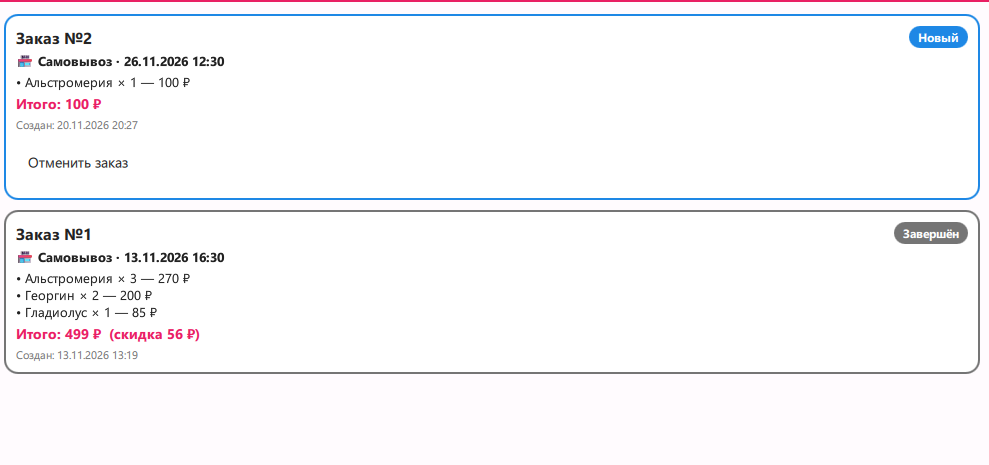
\includegraphics[width=17.0cm,height=0.78\textheight,keepaspectratio]{images/fig19.png}
\caption{История заказов покупателя}\label{fig:3.15}
\end{figure}

Администратор входит с~той же формы под учётной записью с~ролью admin и~видит четыре вкладки. Вкладка «Заказы» (рисунок \ref{fig:3.16}) разработана для оперативной работы: текущие заказы расположены в~порядке наступления назначенного времени, чтобы ближайшие находились вверху. Заказ, срок которого прошёл, помечается как просроченный. Сверху доступен фильтр по статусам с~указанием числа заказов в~каждом. Для каждого заказа выводятся данные покупателя и~контактный телефон, способ получения, время, адрес, состав и~сумма, а~также кнопки: «Взять в~работу», «Заказ готов», «Выдан / доставлен» и~«Отменить заказ».



\begin{figure}[H]
\centering
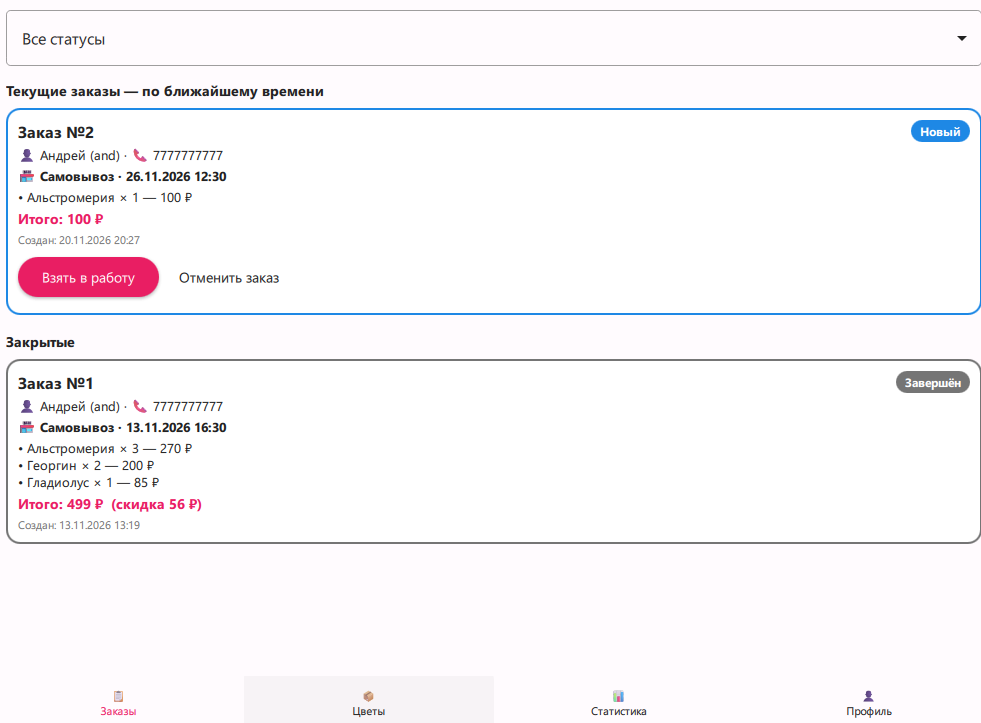
\includegraphics[width=15.5cm,height=0.78\textheight,keepaspectratio]{images/fig20.png}
\caption{Вкладка «Заказы» администратора}\label{fig:3.16}
\end{figure}

Вкладка «Цветы» является складским учётом (рисунок \ref{fig:3.17}). Для каждой позиции показаны фото, цена и~остаток, а~позиции, у~которых осталось не более пяти единиц, выделены красной рамкой. Кнопка редактирования открывает окно изменения цены, количества и~ссылки на фото; отдельная форма позволяет добавить новый цветок с~описанием ухода. Вкладка «Статистика» (рисунок \ref{fig:3.18}) показывает плитки с~ключевыми показателями~– выручкой, числом заказов, числом заказов в~работе, средним чеком, числом покупателей и~видов цветов,~– распределение заказов по статусам, пять самых продаваемых цветов в~виде горизонтальных шкал и~список позиций, которые заканчиваются на складе. Выручка считается по всем заказам, кроме отменённых.



\begin{figure}[H]
\centering
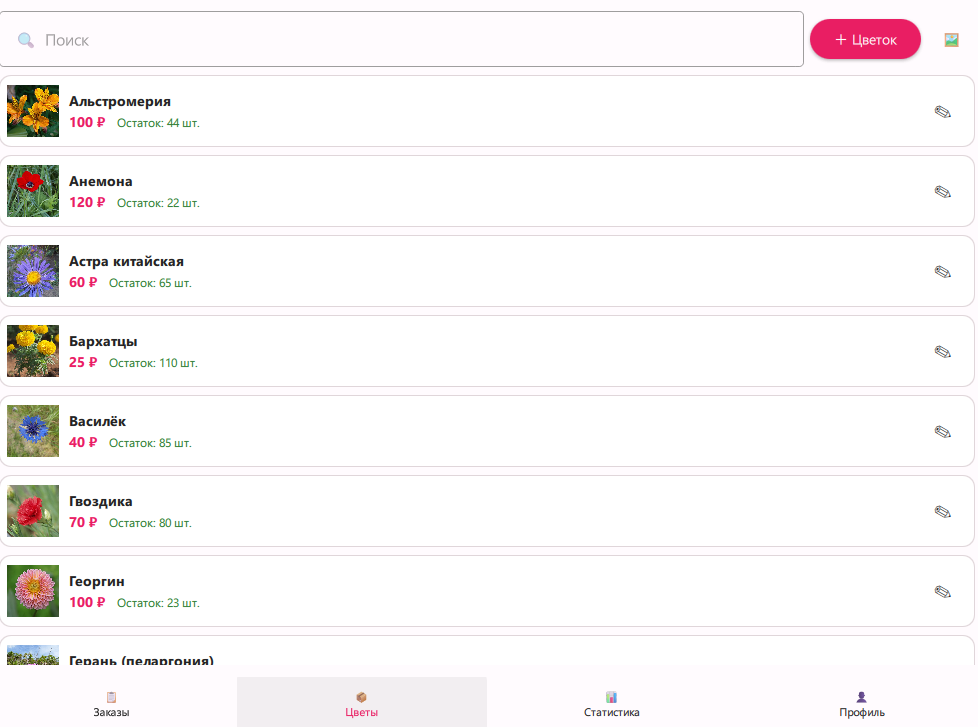
\includegraphics[width=16.5cm,height=0.78\textheight,keepaspectratio]{images/fig21.png}
\caption{Вкладка «Цветы» и~окно редактирования}\label{fig:3.17}
\end{figure}

\begin{figure}[H]
\centering
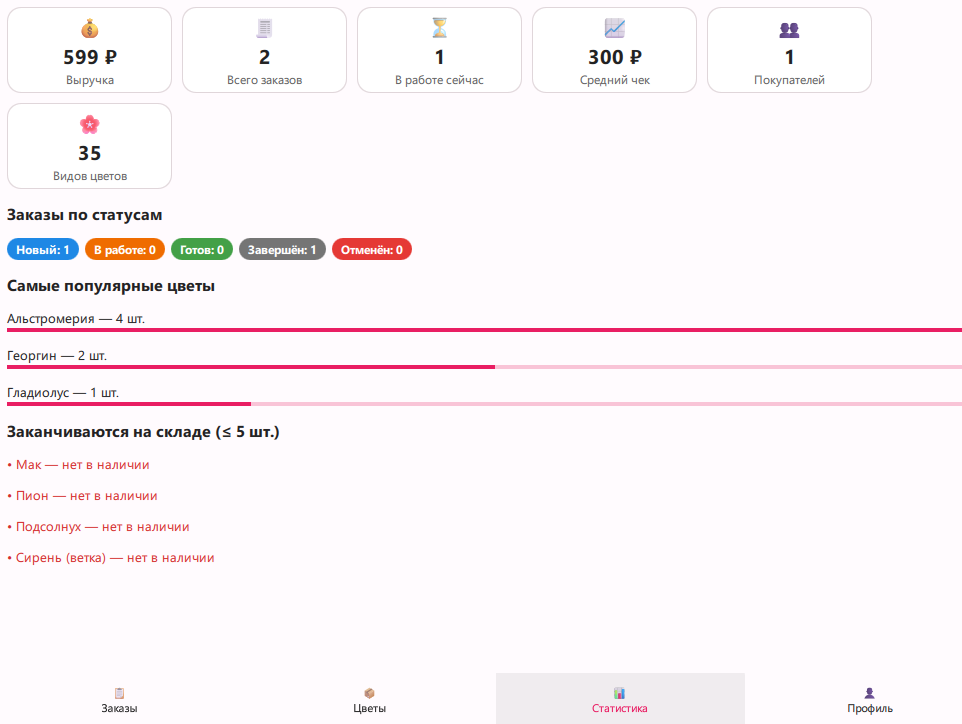
\includegraphics[width=14.7cm,height=0.78\textheight,keepaspectratio]{images/fig22.png}
\caption{Вкладка «Статистика» администратора}\label{fig:3.18}
\end{figure}

\subsection{Работа на нескольких платформах и~альтернативная реализация интерфейса}

Главная особенность приложения~– единая кодовая база для всех платформ. Ни логика, ни интерфейс не содержат веток для конкретной операционной системы: клиентская часть Flet, построенная на Flutter, отрисовывает одинаковые элементы в~окне настольной ОС и~на экране телефона. Различия сведены к~двум вопросам: способу запуска или сборки и~месту хранения файлов приложения \cite{b3}.



Для разработки и~запуска на компьютере достаточно установить зависимости и~запустить файл из среды PyCharm или командой python main.py. Открывается окно размером 1000\ensuremath{\times}780 пикселей с~минимальным размером 360\ensuremath{\times}600, что позволяет проверять и~узкую, «телефонную» компоновку. Основная проверка на настольной платформе выполнялась в~операционной системе Windows; при запуске из среды разработки приложение создаёт базу данных и~загружает фотографии автоматически.



Для получения установочных пакетов используется команда flet build с~указанием целевой платформы: apk или aab для Android, windows, macos или linux для настольных систем. Для сборки требуется Flutter SDK, а~в~документации приведена матрица, показывающая, на какой ОС запускается сборка под конкретную платформу. Параметры сборки заданы в~файле pyproject.toml. Сборка под Android выполняется командой flet build apk; результат помещается в~каталог build/apk проекта и~устанавливается на устройство копированием файла и~открытием его на телефоне. Для быстрой проверки без сборки к~запущенному на компьютере проекту можно подключиться с~помощью приложения Flet на Android-устройстве, находящегося в~одной сети с~компьютером \cite{b3}.



На Android приложение запускается в~изолированной среде, где каталог рядом с~исходным кодом недоступен для записи. Поэтому место хранения базы данных определяется функцией storage\_\allowbreak{}dir: если задана переменная окружения FLET\_\allowbreak{}APP\_\allowbreak{}STORAGE\_\allowbreak{}DATA, которую устанавливает среда исполнения Flet на мобильных платформах, используется её значение, иначе~– каталог data рядом с~программой. Эта единственная платформенная особенность скрыта в~одной функции, а~остальной код работает с~путём как с~обычной строкой.



Адаптивность интерфейса обеспечивается тремя приёмами. Каталог построен на сетке с~максимальной шириной плитки, поэтому число колонок меняется вместе с~шириной окна. Диалоги получают ширину не более 460 пикселей и~не более ширины экрана за вычетом полей. Элементы выбора организованы в~строки, которые делят доступную ширину поровну. Нижняя панель навигации одинаково удобна и~в~окне компьютера, и~на телефоне. Результат на устройстве показан на рисунке \ref{fig:3.19}.



\begin{figure}[H]
\centering
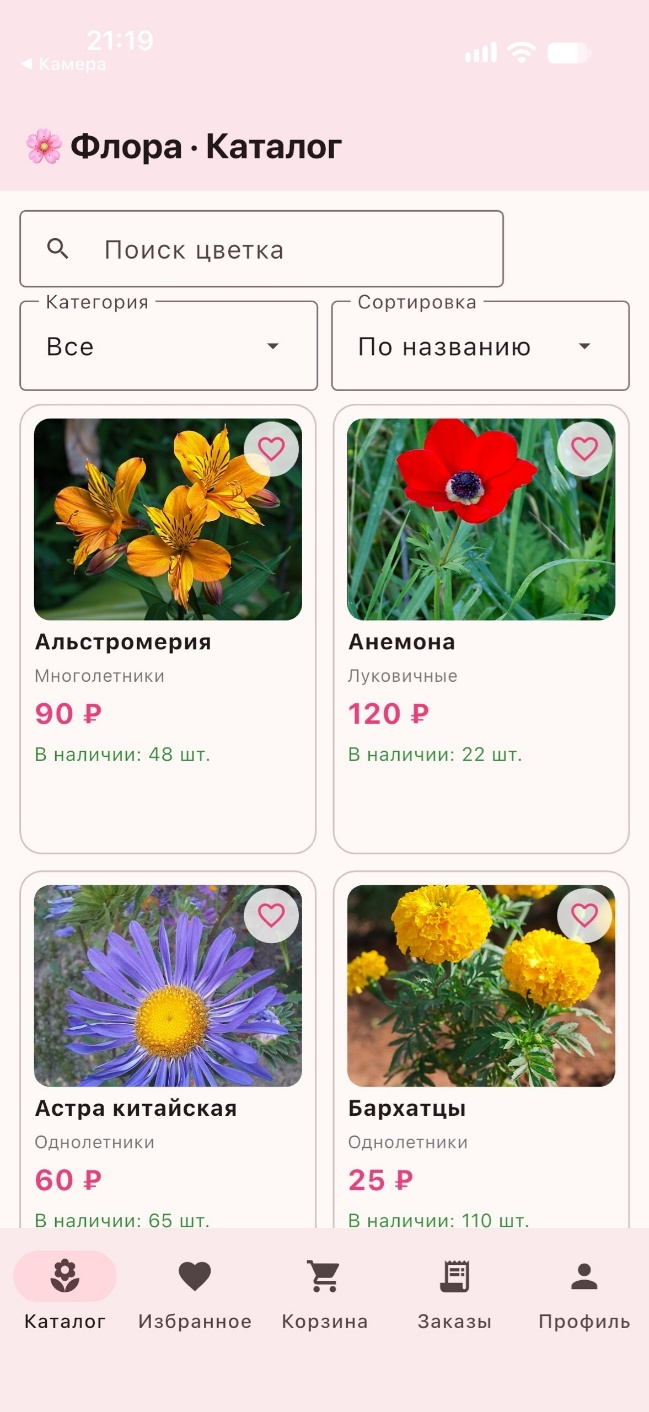
\includegraphics[width=7.4cm,height=0.78\textheight,keepaspectratio]{images/fig23.jpeg}
\caption{Приложение «Флора» на устройстве Android}\label{fig:3.19}
\end{figure}

Чтобы оценить переносимость архитектуры, слой представления был реализован второй раз на технологии Qt Quick: разметка экранов написана на языке QML, а~логика осталась на Python. Модули db.py, photos.py и~flowers\_\allowbreak{}data.py перенесены без изменений, а~заново написаны только 20 файлов QML и~класс Backend~– «мост» между Python и~QML, публикуемый в~интерфейсе методами-слотами и~сигналами \cite{b8}.



Замена слоя представления не потребовала изменений в~логике и~данных, что подтверждает выбранную слоистую архитектуру. В~качестве основной реализации для рассматриваемой задачи принят вариант на Flet как более компактный и~допускающий простую сборку под обе платформы. Проверка QML-варианта на целевых платформах не входила в~объём тестирования настоящей работы.



\subsection{Тестирование приложения}

Тестирование проводилось в~три этапа: автоматические модульные тесты слоя данных, функциональные сценарии для интерфейса и~измерения производительности с~экспертной оценкой удобства. Слой данных содержит основную бизнес-логику~– аутентификацию, заказы, склад и~расчёт стоимости,~– поэтому именно он проверяется автоматически.



Функциональное тестирование интерфейса проводится методом чёрного ящика: проверяется соответствие поведения приложения требованиям без обращения к~коду. Сценарии включают позитивные и~негативные проверки и~опираются на разбиение входных данных на классы эквивалентности и~граничные значения: например, для остатка проверяются значения «0», «меньше остатка» и~«больше остатка», а~для времени~– прошедшее, слишком близкое и~допустимое. Сценарии приведены в~таблице \ref{tab:3.3}, их логическая часть дополнительно подтверждается автоматическими тестами. Для настольной платформы сценарии выполняются в~окне приложения, для Android~– на устройстве после установки APK.



\begingroup\small\singlespacing\setlength{\LTpre}{6pt}\setlength{\LTpost}{10pt}
\begin{longtable}{|>{\centering\arraybackslash}p{\dimexpr 0.0810\textwidth-2\tabcolsep-\arrayrulewidth\relax}|>{\raggedright\arraybackslash}p{\dimexpr 0.4865\textwidth-2\tabcolsep-\arrayrulewidth\relax}|>{\raggedright\arraybackslash}p{\dimexpr 0.4325\textwidth-2\tabcolsep-\arrayrulewidth\relax}|}
\caption{Сценарии функционального тестирования}\label{tab:3.3}\\
\hline
\rowcolor{gray!15}\centering\arraybackslash\bfseries № & \centering\arraybackslash\bfseries Сценарий (шаги) & \centering\arraybackslash\bfseries Ожидаемый результат \\ \hline
\endfirsthead
\hline
\rowcolor{gray!15}\centering\arraybackslash\bfseries № & \centering\arraybackslash\bfseries Сценарий (шаги) & \centering\arraybackslash\bfseries Ожидаемый результат \\ \hline
\endhead
\centering\arraybackslash 1 & Регистрация нового покупателя; повторная регистрация с~тем же логином в~другом регистре; вход с~неверным паролем & Аккаунт создан; во втором случае~– «Такой логин уже занят»; в~третьем~– «Неверный логин или пароль» \\ \hline
\centering\arraybackslash 2 & Вход под admin / admin123 & Открыты вкладки администратора \\ \hline
\centering\arraybackslash 3 & Поиск «тюль», фильтр «Луковичные», сортировка «Сначала дорогие» & Показаны только подходящие цветы в~нужном порядке; при пустом результате~– «Ничего не найдено» \\ \hline
\centering\arraybackslash 4 & Открыть карточку цветка & Видны фото, цена, остаток и~девять блоков информации \\ \hline
\centering\arraybackslash 5 & Открыть карточку «Пион» (остаток 0); попытаться добавить больше остатка у~другого цветка & «Нет в~наличии», кнопка заблокирована; количество ограничено остатком \\ \hline
\centering\arraybackslash 6 & Нажать «{\symfont ♥}» на цветке, открыть «Избранное» & Цветок в~избранном; повторное нажатие убирает его \\ \hline
\centering\arraybackslash 7 & В корзине изменить количество, удалить позицию, ввести промокод SPRING10 и~несуществующий & Сумма пересчитывается; первый код даёт скидку 10 \%, второй~– сообщение «Такого промокода нет» \\ \hline
\centering\arraybackslash 8 & Оформить самовывоз выбрать дату, время, ввести телефон & Заказ создан, показано окно с~номером, открыта вкладка «Заказы» \\ \hline
\centering\arraybackslash 9 & Оформить доставку без адреса; выбрать время ближе чем через 45 минут & Сообщения об ошибке, заказ не создан; такие слоты на сегодня не предлагаются \\ \hline
\centering\arraybackslash 10 & После заказа открыть каталог; отменить новый заказ & Остаток уменьшился на количество в~заказе; после отмены возвращён \\ \hline
\centering\arraybackslash 11 & Администратор провести заказ по статусам до «Завершён»; изменить цену и~остаток; добавить цветок & Статусы меняются последовательно; изменения видны покупателю; новый цветок появляется в~каталоге \\ \hline
\centering\arraybackslash 12 & Администратор открыть «Статистику»; запустить приложение без интернета & Показатели соответствуют заказам; вместо фото~– значки категорий, приложение работает \\ \hline
\end{longtable}\endgroup

Производительность слоя данных измерялась на тестовом компьютере под управлением Linux с~интерпретатором Python 3.12. База данных содержала 35 цветов, замеры усреднялись по нескольким десяткам или сотням повторов (таблица \ref{tab:3.4}). Все операции, кроме проверки пароля, выполняются быстрее одной миллисекунды. Относительно большое время проверки пароля~– следствие защитного механизма: медленное вычисление хэша затрудняет подбор паролей. Вместе с~тем рекомендации OWASP для PBKDF2-HMAC-SHA-256 предполагают не менее 600 000 итераций, а~предпочтительным алгоритмом называют Argon2id. В~приложении применяются 120 000 итераций, что меньше рекомендуемого порога \cite{b6}.



\begingroup\small\singlespacing\setlength{\LTpre}{6pt}\setlength{\LTpost}{10pt}
\begin{longtable}{|>{\raggedright\arraybackslash}p{\dimexpr 0.5741\textwidth-2\tabcolsep-\arrayrulewidth\relax}|>{\raggedright\arraybackslash}p{\dimexpr 0.2407\textwidth-2\tabcolsep-\arrayrulewidth\relax}|>{\centering\arraybackslash}p{\dimexpr 0.1852\textwidth-2\tabcolsep-\arrayrulewidth\relax}|}
\caption{Время выполнения операций слоя данных}\label{tab:3.4}\\
\hline
\rowcolor{gray!15}\centering\arraybackslash\bfseries Операция & \centering\arraybackslash\bfseries Среднее время, мс & \centering\arraybackslash\bfseries Повторов \\ \hline
\endfirsthead
\hline
\rowcolor{gray!15}\centering\arraybackslash\bfseries Операция & \centering\arraybackslash\bfseries Среднее время, мс & \centering\arraybackslash\bfseries Повторов \\ \hline
\endhead
Получение списка всех цветов & 0,20 & \centering\arraybackslash 200 \\ \hline
Поиск с~сортировкой по цене & 0,21 & \centering\arraybackslash 200 \\ \hline
Получение одного цветка по идентификатору & 0,012 & \centering\arraybackslash 500 \\ \hline
Оформление заказа из трёх позиций & 0,97 & \centering\arraybackslash 30 \\ \hline
Расчёт статистики для панели администратора & 0,11 & \centering\arraybackslash 100 \\ \hline
Проверка пароля при входе (PBKDF2, 120 000 итераций) & 31,9 & \centering\arraybackslash 20 \\ \hline
\end{longtable}\endgroup

Удобство интерфейса оценено экспертным методом по эвристикам Нильсена: пользователь получает обратную связь через всплывающие сообщения, цветные статусы заказов и~счётчик корзины; термины и~язык интерфейса привычны; ошибки предотвращаются ограничением количества остатком, выбором времени из списка и~блокировкой кнопок; сообщения об ошибках объясняют причину. К~недостаткам отнесены отсутствие отмены удаления из корзины, маски ввода телефона и~отдельного раздела справки. Поскольку эксперты не являются реальными пользователями, для дальнейшей оценки целесообразно привлечь реальных покупателей. Тексты интерфейса, даты и~суммы приводятся в~привычном российскому пользователю формате.



В ходе разработки и~тестирования выявлено и~устранено два дефекта. Первый (низкая серьёзность) касался внешнего вида: на экране компьютера между строкой поиска и~фильтрами каталога оставалось большое пустое пространство, так как поле поиска в~вертикальной колонке занимало всю свободную высоту; ошибка была устранена удалением соответствующего параметра. Второй касался безопасности: приложение позволяло зарегистрировать логины, отличающиеся только регистром (например, anna и~ANNA), хотя вход выполнялся без учёта регистра; в~функцию создания пользователя добавлена проверка без учёта регистра, после чего все 20 тестов пройдены. Второй дефект наглядно показывает пользу модульных тестов: он не проявлялся при обычной работе с~интерфейсом.



\clearpage

\section*{ЗАКЛЮЧЕНИЕ}\addcontentsline{toc}{section}{ЗАКЛЮЧЕНИЕ}

В ходе выполнения курсовой работы было разработано мультиплатформенное приложение «Флора», предназначенное для просмотра ассортимента и~оформления заказов в~цветочном магазине. Поставленная цель достигнута, основные задачи работы выполнены.



В первой главе были рассмотрены особенности рынка цветов, требования к~приложениям для оформления заказов и~существующие сервисы, включая Flowwow, «Яндекс Цветы» и~«Цветов.ру». Также были изучены подходы к~мультиплатформенной разработке и~методы тестирования программного обеспечения.



Во второй главе проведён анализ инструментов Python для создания пользовательского интерфейса. Рассмотрены Tkinter, Kivy, BeeWare, Qt for Python и~Flet. По результатам сравнения для основной реализации был выбран Flet, для хранения данных~– SQLite, а~для получения изображений использовано API Википедии.



В практической части разработано приложение с~каталогом из 35 видов цветов. Для каждого товара предусмотрены фотографии и~информация об уходе. Реализованы авторизация покупателей и~администратора, корзина, оформление заказов на самовывоз и~доставку, выбор времени получения, избранное, промокоды и~отмена заказов. Администратор может просматривать и~обрабатывать заказы, управлять складскими остатками и~просматривать статистику. Для хранения информации спроектирована база данных из пяти таблиц, а~пароли сохраняются в~виде хэшей со случайной солью.



Приложение поддерживает запуск на компьютере и~подготовку сборки для Android с~использованием единой кодовой базы. Дополнительно была рассмотрена альтернативная реализация интерфейса с~применением PySide6 и~QML.



Проведённое тестирование включало 20 автоматических модульных тестов, проверку основных функциональных сценариев, измерение производительности и~экспертную оценку удобства использования. В~процессе проверки были выявлены и~устранены два дефекта. Полученные результаты подтвердили работоспособность основных возможностей приложения.



Таким образом, разработанное приложение может использоваться как основа собственного цифрового канала продаж цветочного магазина. В~дальнейшем проект можно расширить за счёт добавления серверной части с~общей базой данных, онлайн-оплаты, системы уведомлений и~дополнительных механизмов защиты учётных записей.



\clearpage

\clearpage
\addcontentsline{toc}{section}{СПИСОК ИСПОЛЬЗОВАННЫХ ИСТОЧНИКОВ}
\begingroup\raggedright\singlespacing
\begin{thebibliography}{99}
\bibitem{b1} Appropriate Uses For SQLite : документация SQLite / SQLite Consortium.~– URL: \url{https://www.sqlite.org/whentouse.html} (дата обращения: 21.11.2026).~– Текст : электронный.

\bibitem{b2} BeeWare : документация : [сайт] / BeeWare project.~– URL: \url{https://docs.beeware.org/} (дата обращения: 15.11.2026).~– Текст : электронный.

\bibitem{b3} Flet Documentation : документация фреймворка Flet : [сайт] / Flet Dev.~– URL: \url{https://docs.flet.dev/} (дата обращения: 19.11.2026).~– Текст : электронный.

\bibitem{b4} Flowwow: цветы, подарки, торты : мобильное приложение / FLOWWOW LLC.~– URL: \url{https://apps.apple.com/ru/app/id1201155481} (дата обращения: 16.11.2026).~– Текст : электронный.

\bibitem{b5} MediaWiki Action API : документация / Wikimedia Foundation.~– URL: \url{https://www.mediawiki.org/wiki/API:Main_page} (дата обращения: 21.11.2026).~– Текст : электронный.

\bibitem{b6} Password Storage Cheat Sheet / OWASP Foundation.~– URL: \url{https://cheatsheetseries.owasp.org/cheatsheets/Password_Storage_Cheat_Sheet.html} (дата обращения: 22.11.2026).~– Текст : электронный.

\bibitem{b7} Python 3 Documentation : sqlite3, tkinter и~стандартная библиотека : [сайт] / Python Software Foundation.~– URL: \url{https://docs.python.org/3/} (дата обращения: 14.11.2026).~– Текст : электронный.

\bibitem{b8} Qt for Python (PySide6) Documentation : [сайт] / The Qt Company.~– URL: \url{https://doc.qt.io/qtforpython-6/} (дата обращения: 17.11.2026).~– Текст : электронный.

\bibitem{b9} Анализ рынка срезанных цветов в~России в~2020–2024 гг, прогноз на 2025–2029 гг / BusinesStat // РБК Магазин исследований : [сайт].~– 14 ноября 2025.~– URL: \url{https://marketing.rbc.ru/research/27942/} (дата обращения: 19.11.2026).~– Текст : электронный.

\bibitem{b10} Интернет-торговля в~России в~первом полугодии 2026 года : данные / АКИТ // Ассоциация компаний интернет-торговли : [сайт].~– 2026.~– URL: \url{https://akit.ru/} (дата обращения: 15.11.2026).~– Текст : электронный.

\bibitem{b11} Любанович, Б. Простой Python. Современный стиль программирования / Б. Любанович ; пер. с~англ. Е. В. Зазноба.~– 2-е изд.~– Санкт-Петербург : Питер, 2021.~– 592 с.~– ISBN 978-5-4461-1639-3.~– Текст : непосредственный.

\bibitem{b12} Цветов.ру~– доставка цветов : мобильное приложение.~– URL: \url{https://www.rustore.ru/catalog/app/ru.cvetov.app} (дата обращения: 18.11.2026).~– Текст : электронный.

\bibitem{b13} Яндекс Цветы: доставка букетов : мобильное приложение / ООО «Яндекс».~– URL: \url{https://www.rustore.ru/catalog/app/ru.yandex.flowers} (дата обращения: 20.11.2026).~– Текст : электронный.
\end{thebibliography}
\endgroup
\end{document}
